\renewcommand{\typeRubriek}{loep}		

%%%%%%%%%%%%%%%%%%%%%%%%%%%%%
% informatie voor de auteur %
%%%%%%%%%%%%%%%%%%%%%%%%%%%%%
% de soorten titels opmaakmogelijkheden die de auteur kan gebruiken:
% section
% section*, betekent dat er geen nummer bij gezet wordt
% subsection
% tussentitel
% citaat
% opsomming
% nummering
% bronnen
% kader
% stellingkader (genummerd)
% stellingkadertwee (niet genummerd)
% kleurkader
% werktekst



% twee parameters voor nieuwe rubriek: titel en auteur (die mogen ook leeggelaten worden o.a. voor redactioneel)
\startNieuweRubriek{Gewoon mooie\\ oefeningen}{Els Vanlommel\\ Hilde Eggermont \\Els Van Emelen\\Michel Roelens}
\vspace{1.5cm}
\startcontents[mainsections]		      % om opsomming in inhoudstafel enkel tot loep te beperken




%%%%%%%%%%%%%%%%%%%%%%%%%%%%%%%%%%%%%%%%%%%%%%%%%%%%%%%%%%%%%%%%
%%%%%%%%%%%           START VAN DE TEKST               %%%%%%%%%%
%%%%%%%%%%%%%%%%%%%%%%%%%%%%%%%%%%%%%%%%%%%%%%%%%%%%%%%%%%%%%%%%
\begin{multicols}{2}                      
\inhoudstafelLoep		                  % om inhoudstafel in te voegen
\section{Inleiding}

Inspiratie is een wezenlijk onderdeel van wiskunde-onderwijs. Elke les opnieuw, elke toets, elk proefwerk is een zoektocht naar geschikte en mooie vragen. Met deze loep willen wij hiervoor een beetje inspiratie bieden. Geen speciaal thema deze keer, maar een losse verzameling van oefeningen waarvan wij vinden dat ze mooi zijn. We probeerden voor elk wat wils te vinden, gegroepeerd per graad. Sommige vragen zijn wellicht niet direct geschikt voor jouw leerlingen. Die kunnen misschien dienen als inspiratie voor vragen die wél kunnen. Misschien kan een collega één van de vragen gebruiken: deel ze gerust uit! Of wie weet, misschien is het wel leuk om deze oefeningen zelf te proberen. 

Deze loep gaat niet over ruime onderzoeksonderwerpen (zoals bijvoorbeeld op de wiskunde b-dag) en
niet over oefeningen die nieuwe leerstof aanbrengen. Het zijn geen oefeningen waarvoor je een hele inleidende tekst moet lezen, er is dus geen verduidelijkende context nodig. Het zijn geen oefeningen die in alle handboeken staan (al halen we onze mosterd ook meestal wel ergens en kunnen we niet controleren of het nergens in een handboek staat). De nadruk ligt niet op problem solving (opgaven waar je erg creatief moet zijn en veel heuristieken moet bovenhalen om eraan te kunnen beginnen). Uiteraard vraagt elke goede oefening wel een stukje problem solving, maar de nadruk ligt er niet op.

Wél verzamelden we enkele duidelijke oefeningen over reguliere leerstof  waarmee een stukje differentiatie mogelijk is. De oefening kan bijvoorbeeld gedeeltelijk of volledig opgelost worden; er is meer dan één oplossing of oplossingsmethode mogelijk; na het oplossen kan er nog nagedacht worden over een veralgemening of een variant of \ldots \ De oefeningen zijn bruikbaar in de les, als huiswerk of op een toets (maar de nadruk ligt zeker niet op evaluatie).

In deze loep verloopt de bespreking van een oefening volgens een vast patroon: eerst de opgave, dan de oplossing en tot slot een korte bespreking (\aanh{Waarom is dit een mooie oefening?}). De vraag \aanh{waarom mooi?} is trouwens een goede vraag om aan leerlingen te stellen. Het risico dat ze \aanh{niets} antwoorden, nemen we er dan maar bij.  De oplossing wordt op verschillende manieren beschreven: soms geven we gewoon de oplossing, soms beschrijven we het denkproces en soms doen we verslag van een lessituatie.

We hopen dat deze loep je inspiratie geeft om zelf \aanh{goede oefeningen} te verzamelen of op te stellen. We doen hier dan ook een warme oproep: deel je mooie oefeningen met ons, stuur ze naar de redactie zodat wij ze in één van onze volgende nummers kunnen opnemen. Dat is Uitwiskelen!

\end{multicols}

\section{Eerste graad}
\subsection{Recht evenredige grootheden}

\beginwerktekst{Afstand, snelheid, tijd}

Joris woont op 7 km van school. Hij vindt het best haalbaar om deze afstand met de fiets af te leggen. ’s Morgens fietst hij zo fris als een hoentje met een gemiddelde snelheid van 14 km/h. ’s Avonds is hij al wat vermoeid en lukt het niet meer zo vlot. Maar al bij al komt hij in het totaal toch nog aan een gemiddelde snelheid van 12 km/h. Hoe snel fietst hij ’s avonds?

\eindewerktekst

\tussentitel{Oplossing}
\begin{nummering}
  \item Berekening van de fietstijd 's morgens
%
% \todo[inline]{kan ik een tabel op een vaste insprong laten 
% beginnen? en de hoogte van de rijen wat groter maken?} 
%
\tabulinesep=1.5mm
  \begin{flushleft}
  \begin{tabu} to 0.6\textwidth { | X[c] | X[c] | X[c] | }
   \hline
   Afstand & 14 km & 7 km \\
   \hline
   Tijd  & 1 uur  & 30 min  \\
   \hline
  \end{tabu}
  \end{flushleft}

 \item Berekening van de totale fietstijd 's morgens en 's avonds

  \begin{flushleft}
  \begin{tabu} to 0.8
  \textwidth { | X[c] | X[c] | X[c] | X[c] | }
   \hline
   Afstand & 12 km & 2 km & 14 km\\
   \hline
   Tijd  & 1 uur  & 10 min & 70 min  \\
   \hline
  \end{tabu}
  \end{flushleft}
 
  \item Berekening van de snelheid 's avonds
  
 % Fietstijd ' s avonds = 70 min - 30 min = 40 min
 
  \begin{flushleft}
  \begin{tabu} to 0.8
  \textwidth { | X[c] | X[c] | X[c] | X[c] | }
   \hline
   Afstand & 7 km & 3,5 km & 10,5 km\\
   \hline
   Tijd  & 40 min  & 20 min & 60 min  \\
   \hline
  \end{tabu}
  \end{flushleft}
 De snelheid 's avonds is dus 10,5 km/h.
 \newline
 
\end{nummering}


\tussentitel{Wat maakt deze oefening mooi?}
De opgave is boeiend omdat leerlingen de reflex hebben om deze opgave op te lossen door te redeneren met het rekenkundig gemiddelde. Het rekenkundig gemiddelde houdt echter rekening met slechts één grootheid (bv. aantallen, lengtes, gewichten...). Bij het berekenen van de gemiddelde snelheid spelen echter twee grootheden mee: de afstanden die je aflegt en de tijden die je daarvoor nodig hebt. Bij de snelheden\[v_1=\frac{\triangle x_1}{\triangle t_1} \text{ en } v_2=\frac{\triangle x_2}{\triangle t_2}\]wordt de gemiddelde snelheid \[v_{gem}=\frac{\triangle x_1+\triangle x_2}{\triangle t_1+\triangle t_2}.\]

De onderstaande figuur helpt de leerlingen dit beter te begrijpen:\\

\begin{center}
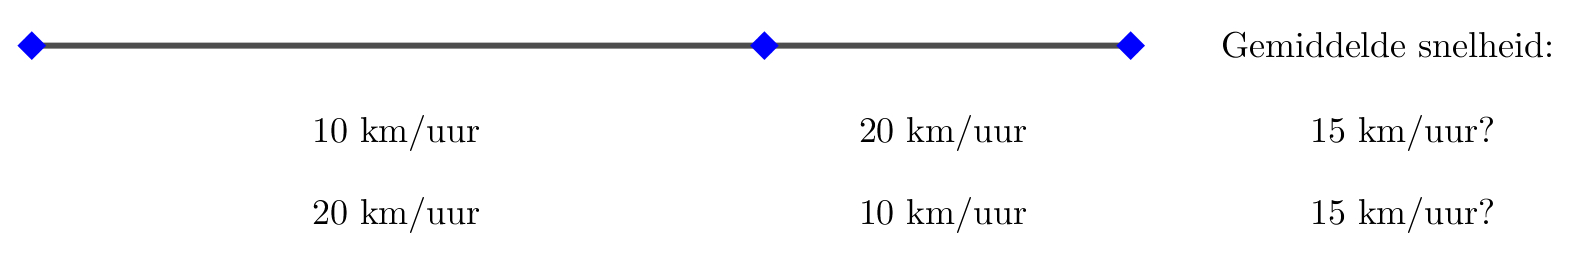
\includegraphics[width=14cm]{img/gemiddeldesnelheid1.jpg}
%\captionof{figure}{}
\end{center}
Voor deze twee gevallen is het duidelijk dat de twee gemiddelde snelheden verschillen. Vaak krijg ik de reactie dat `in dit vraagstuk de afstanden gelijk zijn'. Ik reageer: `Dus als de afstanden verschillen, mag je niet het rekenkundig gemiddelde gebruiken, maar als de afstanden gelijk zijn wel?' Ik vraag hen welke methode ze zouden gebruiken als de afstanden niet gelijk zijn en stel voor om die methode hier ook toe te passen. We grijpen dan terug naar de definitie van gemiddelde snelheid. De leerlingen merken al snel dat deze methode een ander resultaat geeft.  

In de marge: als beide afstanden, zoals hier, toevallig gelijk zijn, wordt de gemiddelde snelheid het harmonische gemiddelde van de twee snelheden:
\begin{align*}
    v_{gem}&=\frac{2 \cdot \triangle x}{\frac{\triangle x}{v_1}+\frac{\triangle x}{v_2}}\\
    &=\frac{2}{\frac{1}{v_1}+\frac{1}{v_2}}.
\end{align*}

\tussentitel{Andere mooie opgaven over afstand - snelheid - tijd}

\begin{opsomming}
\item In een rit van de ronde van Frankrijk wist Tim Wellens te ontsnappen. Toen hij de laatste kilometer aanvatte, waren de achtervolgers 2 km achter hem. Volgens een reporter reden de renners op dat ogenblik (allemaal) 42 km/h en had Wellens een voorsprong van 45 s op zijn achtervolgers. Als de opgegeven snelheid en afstanden correct zijn, kun je het dan eens zijn met de bewering van de reporter? Verklaar. 
\item Twee wielrenners, Arne en Ben, doen mee aan een tijdrit. Arne, die als eerste start, rijdt constant 30 km/h. Ben rijdt 36 km/h. Als Ben start, passeert Arne een kerk. Op het moment dat Arne finisht, passeert Ben diezelfde kerk. Ten slotte finisht Ben precies een half uur na Arne. Hoe lang is het traject van de tijdrit?
\item Een waaghals loopt door een smalle tunnel met slechts één spoor. Op het moment dat hij 40 \% van de tunnellengte achter de rug heeft, hoort hij achter zich in de verte een trein aankomen. Nu kan hij kiezen. Zo hard als hij kan de ene kant oplopen en dan ontsnapt hij ternauwernood aan de trein. Of zo hard als hij kan de andere kant op lopen, en ook dan ontsnapt hij op het nippertje aan een dodelijke botsing. Als de trein met 100 km per uur door de tunnel raast, hoe hard kan die waaghals dan lopen?
\end{opsomming}


\subsection{Meetkunde en massa per volume-eenheid}
\beginwerktekst{Kritisch kijken}

Op het internet vond ik het onderstaande artikel:
\begin{center}
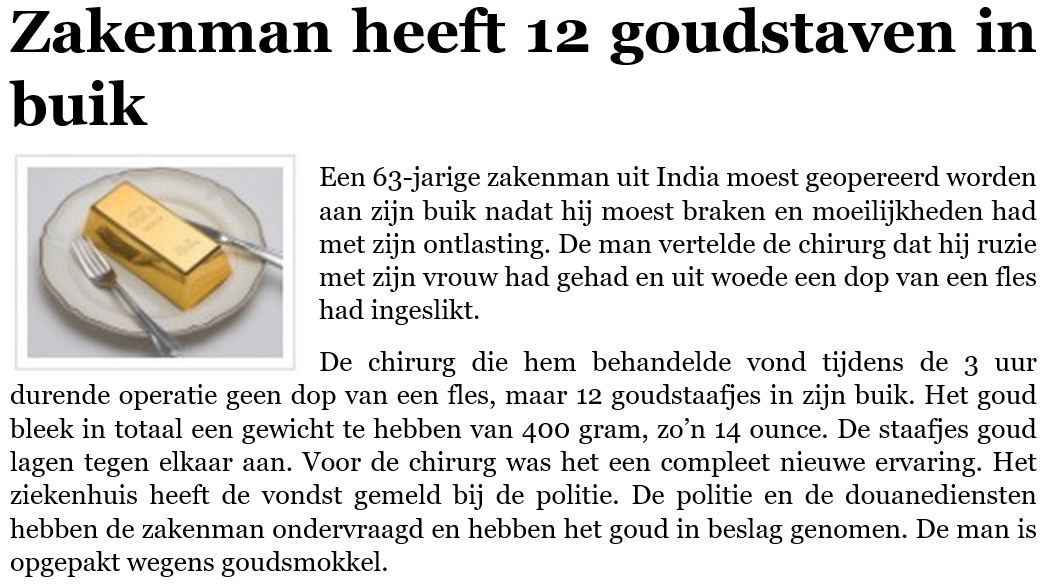
\includegraphics[width=14cm]{img/goudsmokkel.jpg}
\end{center}
\begin{flushright}
\footnotesize{\texttt{https://www.doijerkalff.nl/goud-prijs/goudsmokkel-india/}}
\end{flushright}
\normalsize
Na het lezen van het artikel, had ik bedenkingen bij de foto. Waarom?

\eindewerktekst

\tussentitel{Oplossing}

\textbf {Gegeven} \hspace{6cm} \textbf{Gevraagd}: kritisch kijken naar de foto?
\begin{opsomming}
  \item 12 goudstaven
  \item massa: 400 g = 0,400 kg
  \item massa per volume-eenheid: 19~$ \frac{\textrm{kg}}{\textrm{dm}^3}$
\end{opsomming}


\textbf{Oplossing}:
\begin{nummering}
  \item Massa van 1 staaf $= 0,400~\textrm{kg} : 12 \approx 0,030~ \textrm{kg} $
  \item Volume van 1 staaf
\tabulinesep=1.5mm
   \begin{flushleft}
   \begin{tabu} { | c | c | c| }
     \hline
     Volume & 1 dm$^3$ & ongeveer 0,0015~ dm$^3$ = 1,5 cm$^3$ \\
     \hline
     Massa  & 19 kg  & 0,03 kg  \\
     \hline
  \end{tabu}
  \end{flushleft}
\item Mogelijke afmetingen van 1 staaf met dit volume van 1,5 cm$^3$: 1 cm $\cdot$ 1 cm $\cdot$ 1,5 cm.
\end{nummering}
De staaf op het bord is veel te groot. De staafjes in de buik van de zakenman zijn ongeveer zo groot als een half klontje suiker. Dat is een blokje dat je nog kan doorslikken.


\tussentitel{Wat maakt deze oefening mooi?}
Ik ben altijd argwanend bij foto's of filmpjes met `goudstaven'. De massadichtheid van goud is 19~kg/dm$^3$. Een blokje van 1~dm$^3$ weegt meer dan  een volle emmer water. Dat is erg zwaar in vergelijking met andere stoffen (bv. ijzer weegt 7~kg/dm$^3$). Wiskunde geeft je een middel om dit kritisch in vraag te stellen.


\subsection{Niet recht evenredig}

\beginwerktekst{Door-denken}
\begin{werktekstoef}

\item{Een lift kan 12 volwassenen of 20 kinderen vervoeren. Hoeveel kinderen mogen er maximaal bij 9 volwassenen?}
\item{Om een lange, smalle plank van 3 meter in 3 gelijke plankjes te zagen heeft Michiel 4 minuten nodig. In hoeveel tijd kan hij dezelfde plank in 6 gelijke plankjes zagen?}

\end{werktekstoef}  
\eindewerktekst

\tussentitel{Wat maakt deze oefening mooi?}
Deze oefeningen passen mooi bij het onderwerp recht evenredige grootheden omdat je net niet zomaar de recht evenredigheid kan toepassen. Ze vormen een mooi tegengewicht bij het `automatisch' toepassen van de leerstof.

\tussentitel{Oplossing}
\begin{nummering}
  \item De massa van 12 volwassenen is gelijk aan de massa van 20 kinderen. Als er al 9 volwassenen in de lift staan, zouden er nog 3 bij kunnen. We zoeken met hoeveel kinderen dit overeenkomt.
  \tabulinesep=1.5mm
   \begin{flushleft}
  \begin{tabu} to 0.8\textwidth { | X[c] | X[c] | X[c] |}
   \hline
   Aantal volwassenen & 12 volwassenen& 3 volwassenen  \\
   \hline
   Aantal kinderen  & 20 kinderen  & 5 kinderen \\
   \hline
  \end{tabu}
  \end{flushleft}
   Er kunnen dus nog 5 kinderen bij in de lift.
  \item Bij de tweede opgave helpt het om een schets te maken. Om de plank in 3 stukken te zagen, moeten we twee keer zagen.
    \begin{center}
    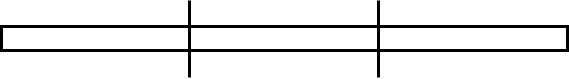
\includegraphics[width=12cm]{img/plank1.jpg}
       \end{center} 
  
  Om de plank in 6 gelijke stukken te zagen moeten we 5 keer zagen.
  \begin{center}
    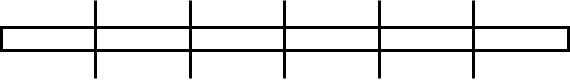
\includegraphics[width=12 cm]{img/plank2.jpg}
    \end{center}
\tabulinesep=1.5mm
    \begin{flushleft}
    \begin{tabu} to 0.9\textwidth { | X[c] | X[c] | X[c] | X[c]|}
    \hline
     Aantal zaagsneden & 2 sneden & 1 snede & 5 sneden  \\
    \hline
     Tijd  & 4 min & 2 min & 10 min  \\
    \hline
    \end{tabu}
    \end{flushleft}
    
\end{nummering}


\subsection{Veelvouden, delers en restbepaling}

\beginwerktekst{Knikkers verdelen}

Er staat een emmer vol knikkers. Je neemt telkens 8 knikkers tot je nog maar 7 knikkers overhoudt. Je doet alle knikkers terug in de emmer. Dan neem je er telkens 7 uit. Je houdt nu uiteindelijk 6 knikkers over. Weer doe je de knikkers terug in de emmer. Vervolgens neem je er telkens 6 uit en hou je er 5 over. Zo ga je door tot je er telkens 2 uit gehaald hebt en er 1 overblijft. Wat is het kleinste aantal knikkers dat er in de emmer kan zitten?

\eindewerktekst
\vspace{-0.7cm}
\tussentitel{Wat maakt deze oefening mooi?}
Het is een opgave met een lage instap en ze past in problem solving. Je kunt er met relatief weinig voorkennis aan beginnen. Tijdens het zoeken ervaar je hoe wiskunde, door het zoeken naar patronen, helpt om te vereenvoudigen en te structureren. Het is een opgave waarbij wroeten nodig is als je de opgave niet meteen doorziet. Het prettige is dat voortschrijdend inzicht je telkens opnieuw een stapje verder helpt. 
Ik geef daarom hieronder niet zomaar de oplossing maar maak het denken van `een leerling' zichtbaar. Ik toon hoe het voortschrijdend inzicht hem telkens verder helpt om de oplossing te vinden. Er zijn natuurlijk nog andere manieren om de oplossing te vinden.
Het is een opgave waar je de leerlingen zelfstandig (eventueel in groepjes) aan kunt laten werken en hen telkens opnieuw een hint kunt geven. Op die manier zet je in op het ontdekken van nieuwe patronen. Zelf probeer ik om zo weinig mogelijk te verklappen en vooral kritische waarom-is-dat-zo-vragen te stellen. Wanneer je deze patronen laat verklaren komen er heel wat eigenschappen naar boven.
\tussentitel{Oplossing}
De opgave geeft in eerste instantie veel wanorde in mijn hoofd. Het lijkt alsof ik met heel veel parameters rekening moet houden. Ik ken enkele regels van restbepaling (door 4, door 3, door 5 en door 2) maar die helpen me niet direct verder, behalve dat ik besef dat het getal dat ik zoek oneven moet zijn. Ik probeer inzicht te krijgen hoe de resten evolueren voor de verschillende delers. Ik start met het getal 15 omdat dit het eerste getal is dat een rest van 7 geeft als ik deel door 8.
%\todo[inline]{kan ik in deze tabel ook de grootte van de hokjes specifieren en dan toch centeren van de inhoud?}
  \begin{flushleft}
  \begin{tabular}{ | m{3cm} | >{\centering\arraybackslash}m{1cm} | >{\centering\arraybackslash}m{1cm} | >{\centering\arraybackslash}m{1cm} | >{\centering\arraybackslash}m{1cm} | >{\centering\arraybackslash}m{1cm} | >{\centering\arraybackslash}m{1cm} | >{\centering\arraybackslash}m{1cm} |  } 
  \hline
  Rest bij deling door & 8 & 7 & 6 & 5 & 4 & 3 & 2 \\ 
  \hline
  15 & 7 & 1 & 3 & 0 & 3 & 0 & 1  \\ 
  \hline
  \end{tabular}
  \end{flushleft}
Ik vul dit aan met nieuwe getallen om zicht te krijgen op hoe de resten veranderen. Ik kies een tweede getal waarbij ik de rest van 7 bij deling door 8 wil behouden. Zo vind ik het getal 23 (= 15 + 8). Daarna blijf ik er telkens 8 bij optellen en zoek naar een patroon in de resten. 
  \begin{flushleft}
  \begin{tabular}{ | m{3cm} | >{\centering\arraybackslash}m{1cm} | >{\centering\arraybackslash}m{1cm} |>{\centering\arraybackslash}m{1cm}| >{\centering\arraybackslash}m{1cm}| >{\centering\arraybackslash}m{1cm}| >{\centering\arraybackslash}m{1cm}| >{\centering\arraybackslash}m{1cm}|  } 
  \hline
  Rest bij deling door & 8 & 7 & 6 & 5 & 4 & 3 & 2 \\ 
  \hline
  15 & 7 & 1 & 3 & 0 & 3 & 0 & 1  \\ 
   \hline
  23 & 7 & 2 & 5 & 3 & 3 & 2 & 1  \\
  \hline
  31 & 7 & 3 & 1 & 1 & 3 & 1 & 1  \\
  \hline
  39 & 7 & 4 & 3 & 4 & 3 & 0 & 1  \\
  \hline
  47 & 7 & 5 & 5 & 2 & 3 & 2 & 1  \\
  \hline
  55 & 7 & 6 & 1 & 0 & 3 & 1 & 1  \\ 
  \hline
  \end{tabular}
  \end{flushleft}
Terwijl ik de resten bereken, vallen een aantal dingen op:
\begin{opsomming}
  \item Alle getallen geven rest 1 bij deling door 2. Dat had ik al bedacht want als je bij een oneven getal een even getal optelt, blijft dat oneven.
  \item Ik zie dat de rest bij deling door 7 telkens eentje meer wordt. Dat is ook logisch. Je telt er 8 bij, als je deelt door 7 is de rest eentje hoger geworden. 
  \item Ik zie ook dat de rest bij deling door 4 niet verandert. Gelukkig is die 3, wat één van de voorwaarden was. Dat komt doordat 4, en ook 2, delers zijn van 8. Als je er 8 bij optelt, verandert de rest niet bij deling door 2 en 4.
  \end{opsomming}

Bij 55 heb ik een getal gevonden dat bij deling door 8 rest 7 geeft en bij deling door 7 rest 6. Dat wil ik graag zo houden.

Opnieuw stotteren mijn gedachten door de veelheid van parameters die ik in het oog moet houden. Ik vraag me af waarom het 55 is. Natuurlijk, dat is $7 \cdot 8 - 1$. Dus als ik dit wil behouden moet ik een veelvoud van $7 \cdot 8$ optellen. Ik probeer verder...
  \begin{flushleft}
  \begin{tabular}{ | m{3cm} | >{\centering\arraybackslash}m{1cm}| >{\centering\arraybackslash}m{1cm} |>{\centering\arraybackslash}m{1cm}| >{\centering\arraybackslash}m{1cm}| >{\centering\arraybackslash}m{1cm}| >{\centering\arraybackslash}m{1cm}| >{\centering\arraybackslash}m{1cm}|  } 
  \hline
  Rest bij deling door & 8 & 7 & 6 & 5 & 4 & 3 & 2 \\ 
   \hline
  ... &  &  &  &  &  &  &   \\ \hline
  55 & 7 & 6 & 1 & 0 & 3 & 1 & 1  \\
  \hline
  111 &  &  & 3 &  &  &  &   \\
  \hline
  167 &  &  & 5 &  &  &  &   \\ 
  \hline
  \end{tabular}
  \end{flushleft}
Ik raak gefrustreerd over al dat rekenen en probeer het over een andere boeg te gooien. Het getal dat ik zoek, ziet er als volgt uit: 
\[x=n \cdot 8+7=p \cdot 7+6=q \cdot 6+5=r \cdot 5+4= s \cdot 3+2\]
Dat zijn wel heel veel vergelijkingen en onbekenden. Dit stelsel oplossen helpt me niet verder. Wat me wel opvalt is dat 
\[q \cdot 6+5= (q \cdot 6+3)+2= s \cdot 3+2\]

Dat betekent dat als er voldaan is aan een rest van 5 bij deling door 6, er automatisch ook voldaan is aan de voorwaarde bij deling door 3. Gelukkig, ik hoef dus niet langer te piekeren over 2, 3 en 4.

Deze laatste redenering helpt me om op een andere manier naar het getal 167 te kijken.
\[167 = (7 \cdot 8) - 1 + 2 \cdot (7 \cdot 8)= 3 \cdot (7 \cdot 8) -1= 3\cdot7\cdot8-1\]

Deze stap betekent een doorbraak (wat een gelukzalig gevoel!). Plots besef ik dat ik het kleinste gemeenschappelijk veelvoud van de getallen 8, 7, 6 en 5 moet berekenen en daar 1 vanaf moet trekken. Ik hoef dus alleen nog te vermenigvuldigen met 5:

\[839 = 2 \cdot 3 \cdot 4 \cdot 5 \cdot 7 -1\]
Achteraf gezien, een eenvoudige oplossing. 

%\todo[inline]{bron nog toevoegen, hoe doe ik dat? https://rekenbeter.wordpress.com/2011/11/15/doordenker-260/}
%\newpage
\subsection{Hoeken}

\beginwerktekst{Verbanden tussen hoeken}

Bekijk de figuur hieronder. De rechten $a$ en $b$ zijn evenwijdig. Welk verband is er tussen de hoeken $\alpha$ en $\beta$ ?
  \begin{center}
  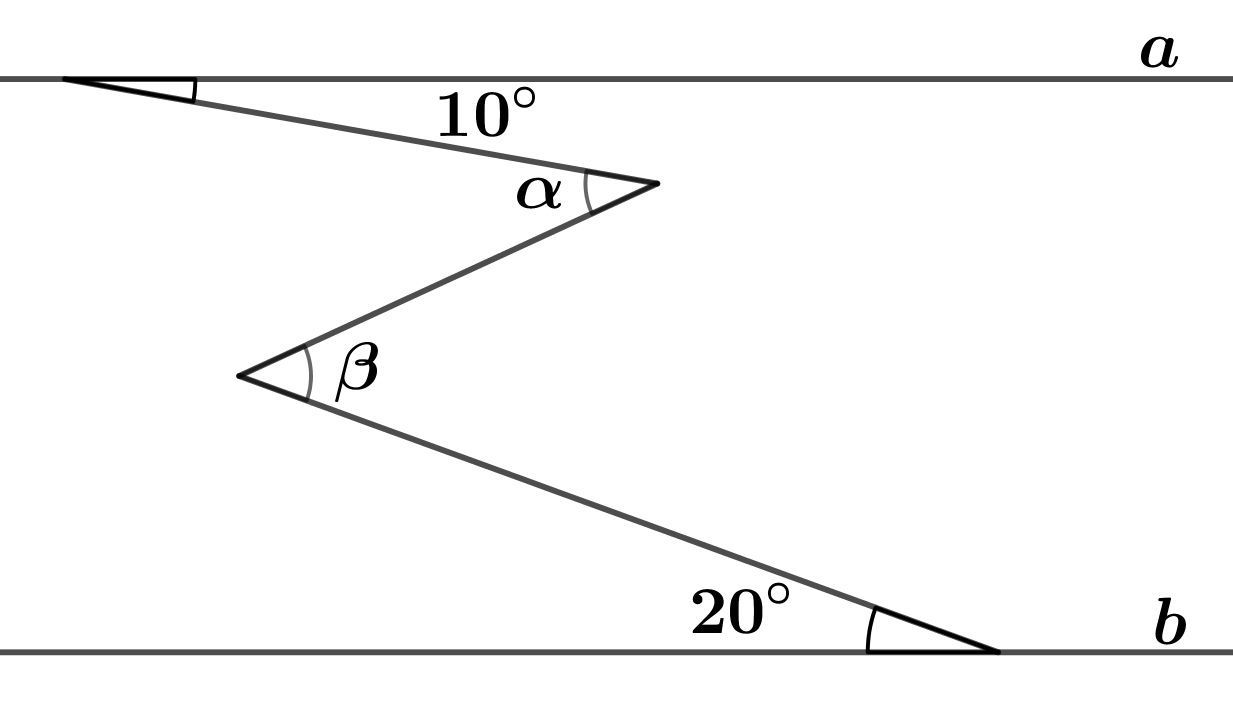
\includegraphics[width=0.4\linewidth]{img/hoeken.jpg}
  \end{center}
\eindewerktekst

\tussentitel{Oplossing}
Teken door de hoekpunten van $\alpha$ en $\beta$ rechten die evenwijdig zijn met $a$ en $b$. Dan wordt $\alpha$ verdeeld in een hoek van 10° (wegens verwisselende binnenhoeken) en een hoek van $\alpha -10$°. De hoek $\beta$ wordt verdeeld in een hoek van 20° en een hoek van $\beta -20$°. Nogmaals door verwisselende binnenhoeken geldt: $\alpha -10$°$=\beta -20$°. Het gevraagde verband is dus $\beta -\alpha=10$°.

\tussentitel{Wat maakt deze oefening mooi?}
De vraag is een beetje ongewoon: er wordt niet gevraagd hoe groot de hoeken zijn maar welk verband ertussen is. Misschien moet vooraf gezegd worden dat de figuur niet \aanh{vastligt} en dat de hoeken van 10° en  20° niet correct getekend zijn. Voor de leerlingen effectief beginnen te rekenen, kun je hen vragen om een andere tekening te maken die ook voldoet aan de gegevens. Ze zien dan dat het onmogelijk is om te weten hoe groot de hoeken apart zijn. Het idee van dingen die veranderen waarbij toch iets \aanh{invariant} blijft, is een belangrijk idee in de (ook veel hogere) wiskunde.
Behalve op het einde een term van lid veranderen, is dit een oefening over één enkel begrip, namelijk verwisselende binnenhoeken. Toch is het een moeilijke oefening omdat er iets moet worden bijgetekend.
Andere oplossingen, bv. steunend op de som van de hoeken in driehoeken (die je maakt door lijnen door te trekken), zijn zeker mogelijk.

\subsection{Oppervlakte}

\beginwerktekst{Verhoudingen van oppervlaktes}

Bepaal de verhouding van de oppervlakte van de driehoek $BMG$ tot de oppervlakte van de regelmatige zeshoek.
 \begin{center}
  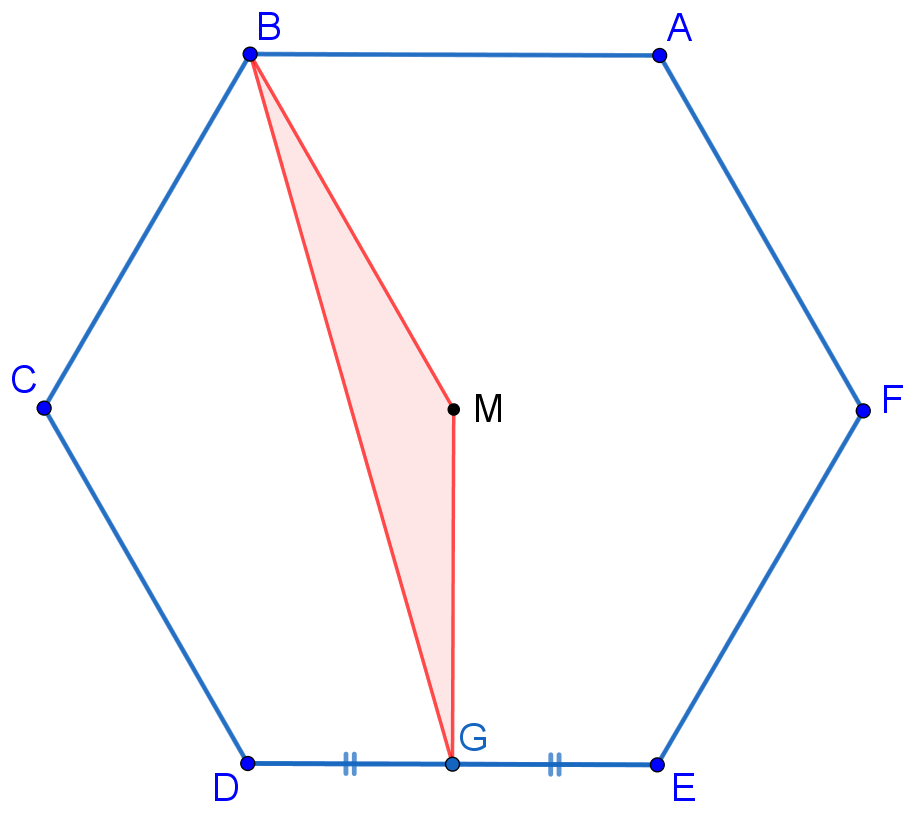
\includegraphics[width=5.5cm]{img/zeshoek01.jpg}
  \end{center}
\eindewerktekst

\tussentitel{Oplossing}

De oppervlakte van de driehoek $BMG$ is gelijk aan de oppervlakte van de driehoek $DMG$. Immers, als we $[MG]$ als basis kiezen, hebben ze dezelfde basis en dezelfde hoogte (linkse figuur). De oppervlakte van de driehoek $BMG$ is dus één twaalfde van de oppervlakte van de zeshoek.
 \begin{center}
  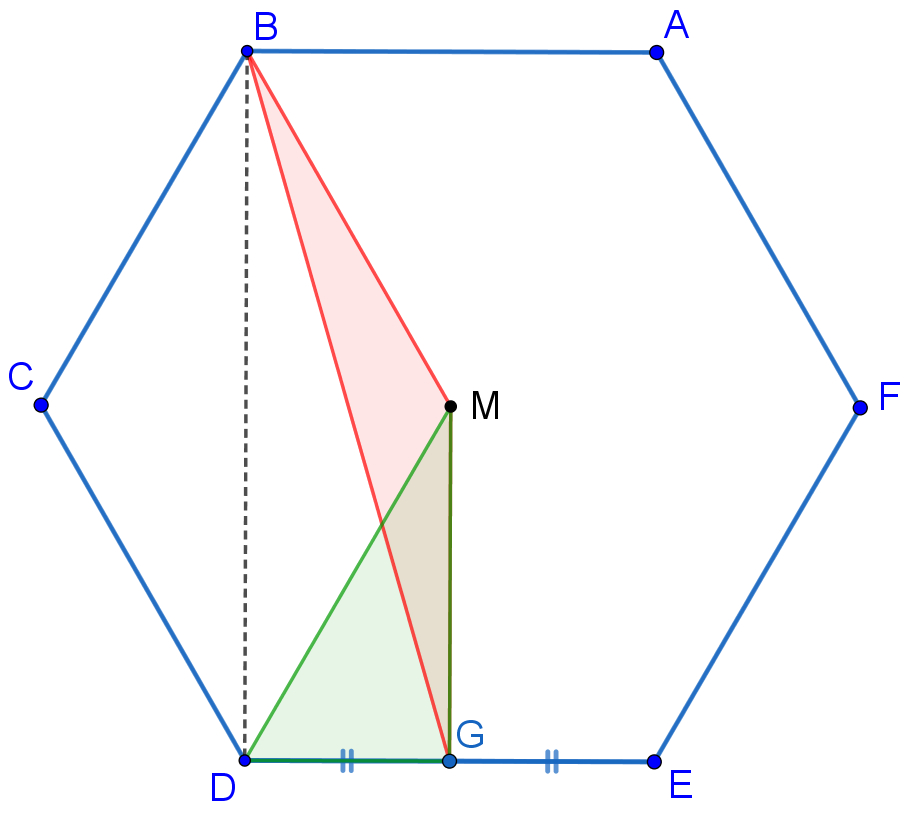
\includegraphics[width=5.5cm]{img/zeshoek02.jpg} \hspace{1cm} 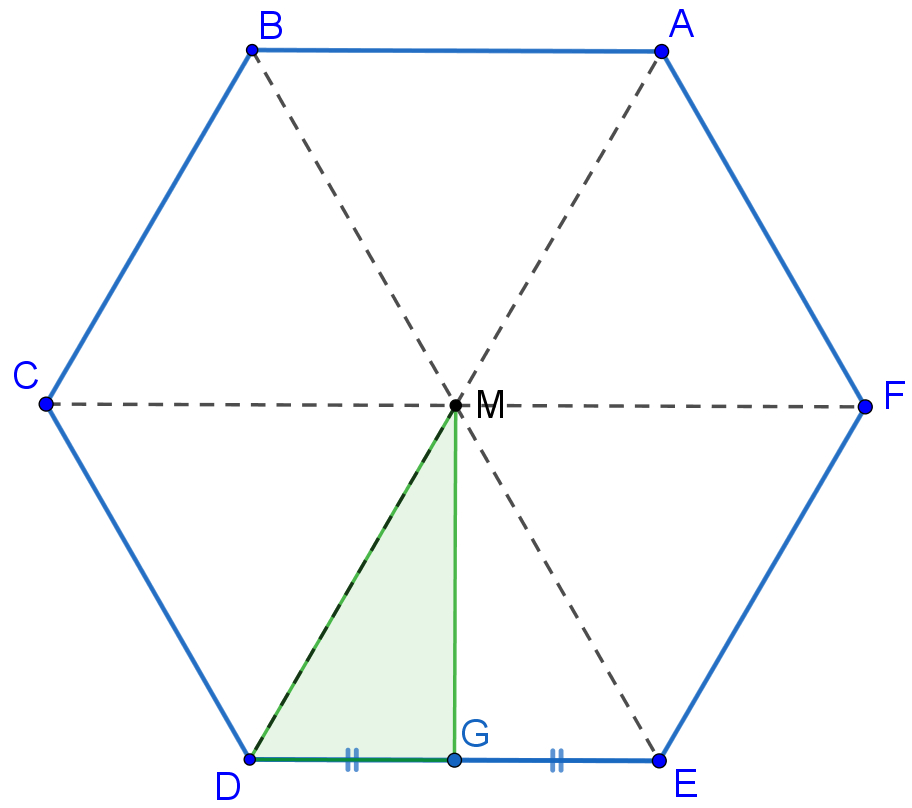
\includegraphics[width=5.5cm]{img/zeshoek03.jpg}
  \end{center}

\tussentitel{Wat maakt deze oefening mooi?}
Bij de oppervlakte van een driehoek is het belangrijk te beseffen dat je steeds \aanh{kiest} wat de basis is, en dat de hoogte na die keuze vastligt (loodrechte afstand van het overstaande hoekpunt tot de drager van de basis). Hier heb je dit echt nodig om de oefening op te lossen. Kies je $[BG]$ als basis, dan lukt het niet met leerstof eerste graad…
Een regelmatige zeshoek mag al eens opduiken v\'o\'or het hoofdstuk \aanh{regelmatige veelhoeken} van de tweede graad. Dit gebeurt trouwens ook vaak bij breuken, als afwisseling bij de (ronde) taarten en pizza’s…

\section{Tweede graad}

\subsection{Stelling van Pythagoras en gelijkvormige driehoeken}

\beginwerktekst{Een vouw in een blad}
\begin{werktekstoef}
\item Een rechthoekig blad papier met lengte 12 cm en breedte 9 cm wordt schuin in twee geplooid zodanig dat de hoek linksboven precies op de hoek rechtsonder valt. Vouw het blad terug open. Hoe lang is de vouw die je net gemaakt hebt?
\begin{center}
\includegraphics[width=2.5cm]{img/vouw1a.png}\ \ 
\includegraphics[width=2.5cm]{img/vouw1b.png}
\end{center}
\end{werktekstoef}

\eindewerktekst
\tussentitel{Oplossing}
Een vouwlijn is steeds de middelloodlijn van twee punten die bij het vouwen op elkaar gelegd worden. In de dichtgevouwen positie is het immers duidelijk dat alle punten van de vouwlijn even ver van beide (samenvallende) punten liggen. Aangezien deze afstanden niet veranderen bij het terug openvouwen, is de vouwlijn inderdaad de middelloodlijn. 

We tekenen de rechthoek en benoemen de punten (zie figuur). We tekenen ook de diagonaal $[BD]$ en de middelloodlijn op deze diagonaal. 

\begin{center}
\includegraphics[width=7cm]{img/vouw2.png}
%\captionof{figure}{Lengte van de vouw}
\end{center}
De lengte van de vouw $[GE]$ noemen we $x$.
Met Pythagoras berekenen we nu de lengte van de diagonaal. We vinden hiervoor $\lvert BD \rvert = 15$.

Verder zijn de driehoeken $ABD$ en $MGD$ gelijkvormig. Beide driehoeken zijn immers rechthoekig en de scherpe hoek in $D$ is gemeenschappelijk. Dit geeft 

\[\frac{\frac{x}{2}}{9}=\frac{7,5}{12}. \]

En dus is $x=\frac{45}{4}.$ 

De vouw is dus 11,25 cm lang.
\vspace{4cm}
\begin{center}
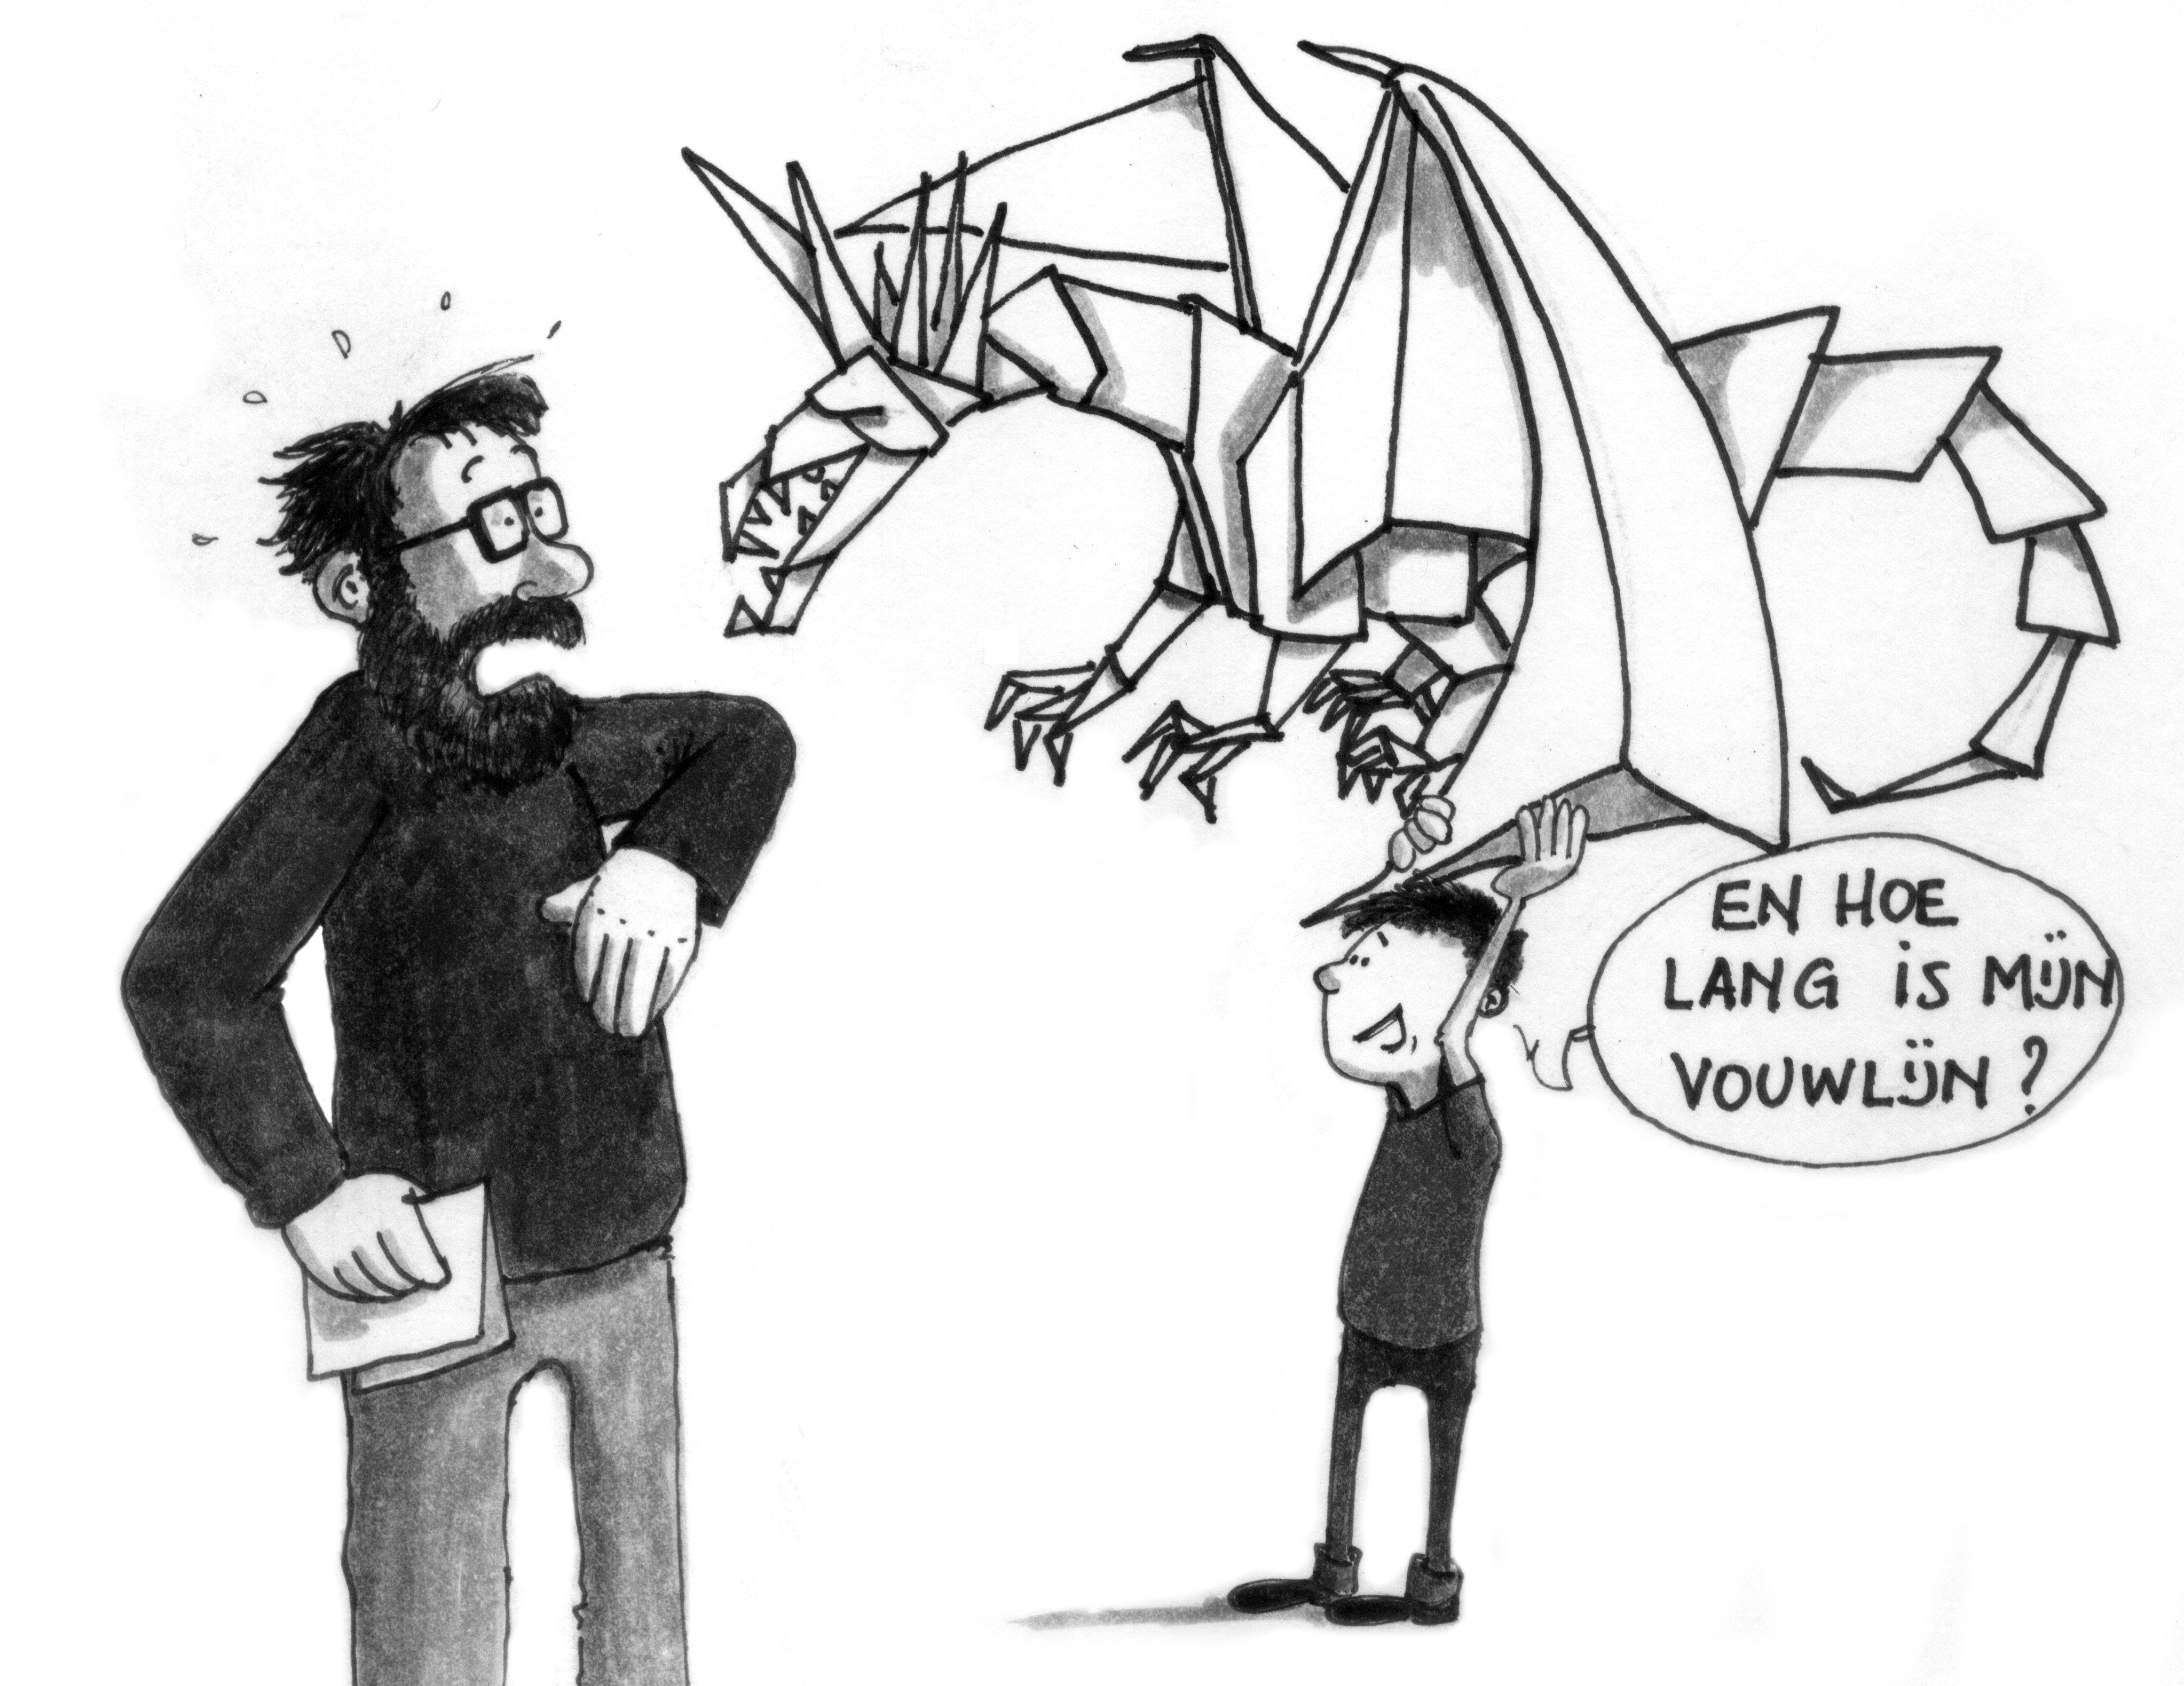
\includegraphics[width=15cm]{img/vouwlijn.jpg}
\end{center}
\tussentitel{Wat maakt deze oefening mooi?}

De vraagstelling is heel eenvoudig. Het is niet moeilijk om je het probleem voor te stellen. Je kunt de leerlingen het probleem voorschotelen zonder figuur, maar door ze een echt blad in twee te laten vouwen. Het maken van een goede tekening is dan een eerste belangrijke stap in de oplossing. De volgende hindernis is het mathematiseren van het vouwen. Tot slot is er nog het probleem van het zien van gelijkvormige driehoeken. Dit is altijd lastiger als die zoals hier elkaar overlappen en niet in dezelfde ‘stand’ staan. 




\subsection{Rijen}
\beginwerktekst{Figuren met lucifers}


Hieronder zijn drie figuren afgebeeld die je met lucifers kunt vormen. De eerste figuur is een vierkant en bestaat uit 4 lucifers; voor de tweede figuur zijn daar 3 lucifers aan toegevoegd en krijg je twee vierkanten tegen elkaar bestaande uit 7 lucifers in het totaal. Je zet deze procedure steeds verder. Je krijgt een steeds langere strook vierkanten. 

\begin{center}
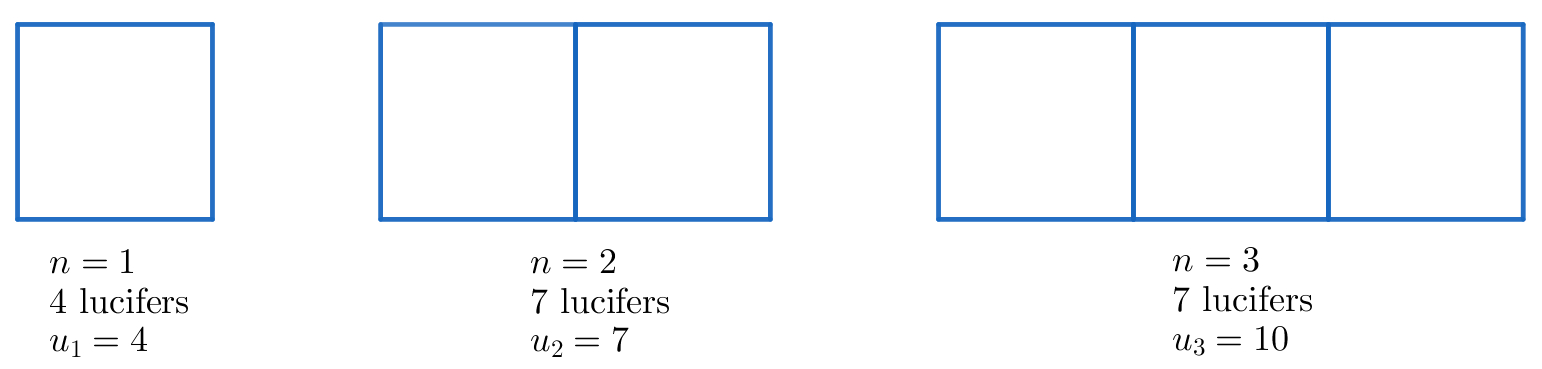
\includegraphics[width=12cm]{img/lucifers01.jpg}
%\begin{tabular}{ m{3cm} m{3cm} m{3cm} }
% 4 lucifers & 7 lucifers & 11 lucifers \\ 
% $u_1 = 4$ & $u_2 = 7$ & $u_3 = 10$
%\end{tabular}
%\captionof{figure}{}
\end{center}

Stel met $u_n$ het aantal lucifers voor dat nodig is om de $n$-de figuur te leggen.
\begin{werktekstoef}
\item Bereken $u_4$.
\item Geef een recursief voorschrift voor $u_n$.
\end{werktekstoef}  

We leggen nu de strookjes met vierkanten tegen elkaar. Waar de strookjes tegen elkaar geschoven zijn, liggen nu telkens twee lucifers tegen of op elkaar.

\begin{center}
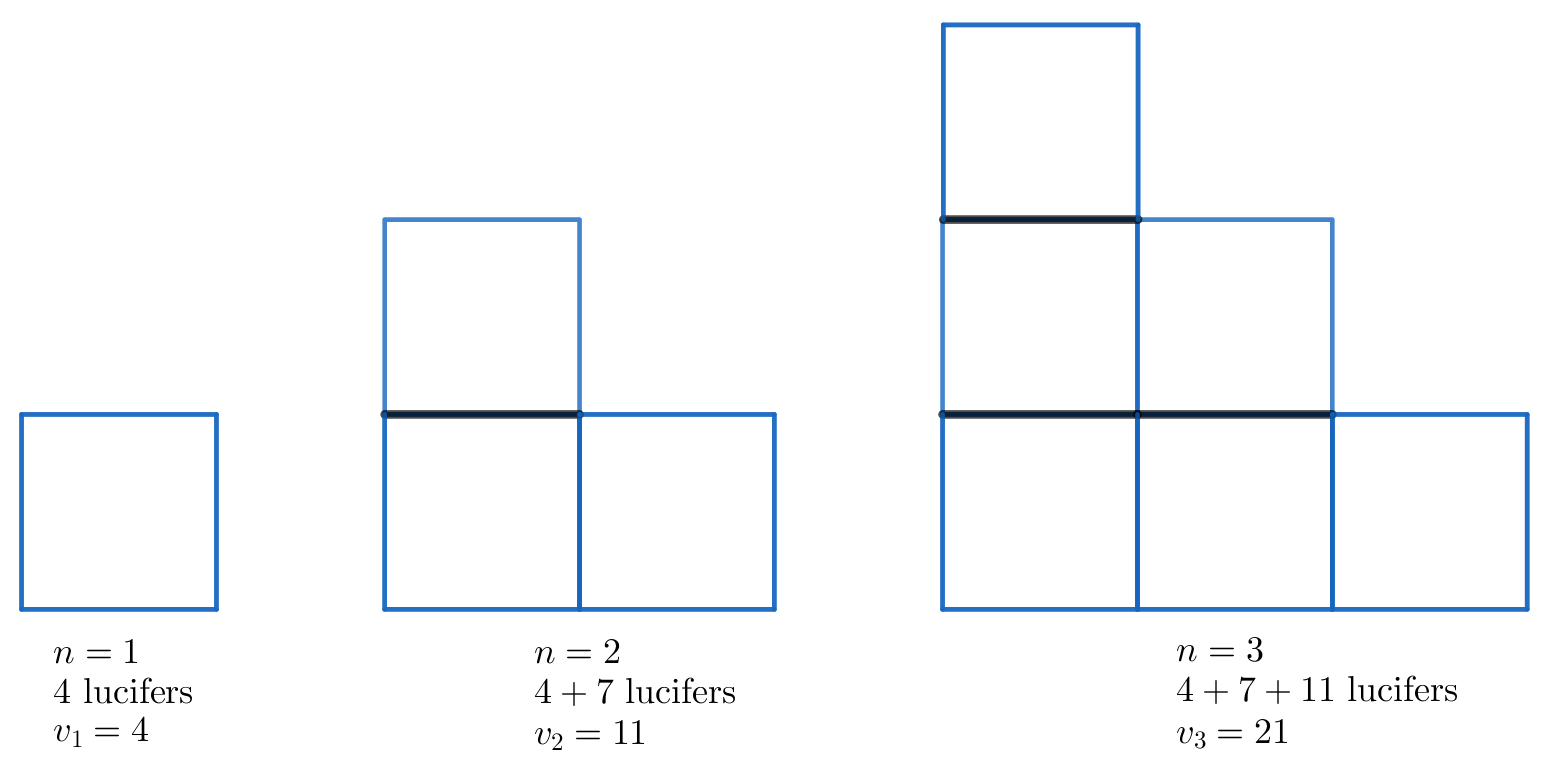
\includegraphics[width=12cm]{img/lucifers02.jpg}
%\begin{tabular}{ m{3cm} m{3cm} m{3cm}  }
% 4 lucifers & $4+7$ lucifers & $4+7+11$ lucifers \\ 
% $v_1 = 4$ & $v_2 = 11$ & $v_3 = 21$
%\end{tabular}
%\captionof{figure}{}
\end{center}

De tweede figuur van deze rij bestaat dus uit $4+7=11$ lucifers. Stel met $v_n$ het aantal lucifers voor in de $n$-de figuur van deze rij figuren. 


\begin{werktekstoef}
\setcounter{enumi}{2}
\item{}
Stel een expliciete formule op voor $v_n$.
\end{werktekstoef}
Waar er twee lucifers tegen elkaar liggen, halen we er nu telkens één weg. In de eerste figuur moet je niets weghalen, in de tweede 1 lucifer en in de derde 3 lucifers.
\begin{werktekstoef}
\setcounter{enumi}{3}
\item Hoeveel lucifers moet je weghalen in de $n$-de figuur?
\end{werktekstoef}
Nu we de dubbels hebben weggehaald, bestaat de eerste figuur nog altijd uit 4 lucifers, maar de tweede uit 10, de derde uit 18, enz. 
Stel met $w_n$ het aantal lucifers voor in de $n$-de figuur na het weghalen van de dubbels. Dan is $w_1=4$, $w_2=10$, $w_3=18$, enz. 

\begin{werktekstoef}
\setcounter{enumi}{4}
\item Stel een expliciete formule op voor $w_n$.
\item De hoeveelste figuur van de rij $w_n$ kun je leggen met 990 lucifers?
\end{werktekstoef}
\eindewerktekst

\tussentitel{Oplossing}

\begin{nummering}
\item	$u_4=10+3=13$
\item	$u_n=u_{n-1}+3$   en  $u_1=4$

De rij $u_n$ is een rekenkundige rij.
\item $\displaystyle v_n=u_1+u_2+ \cdots +u_n = n\cdot \frac{u_1+u_n}{2}= n \cdot \frac{4+4+3(n-1)}{2} = \frac{n \cdot (3n+5)}{2}$
\item $\displaystyle 0+1+2+ \cdots +(n-1)=\frac{n(n-1)}{2}$
\item	$\displaystyle w_n=v_n-\frac{n(n-1)}{2}=\frac{n \cdot (3n+5)}{2}- \frac{n(n-1)}{2} = \frac{2n^2+6n}{2} = n^2+3n$
\item	Hiervoor lossen we de vierkantsvergelijking $n^2+3n-990=0$ op. Die heeft $30$ en $-33$ als oplossingen. Omdat $n$ een natuurlijk getal moet zijn, vinden we $n=30$.
\end{nummering}

\tussentitel{Wat maakt deze oefening mooi?}

In het vierde jaar ligt de focus (zeker bij de oefeningen) heel vaak op rekenkundige en meetkundige rijen. Hierdoor beseffen leerlingen niet (meer) dat er ook andere rijen bestaan. Het is voor hen lastig om (partieel-)sommen als een nieuwe rij te bekijken. 




\subsection{Differentiequotiënt}

\beginwerktekst{De joggers}

Hieronder zie je de grafiek van twee joggers, An en Britt, die hetzelfde parcours lopen. Op de horizontale as staat de tijd $t$ in uren, op de verticale as de afgelegde afstand $s$ in km. Zoals je ziet, vertrekt Britt later dan An.
\begin{center}
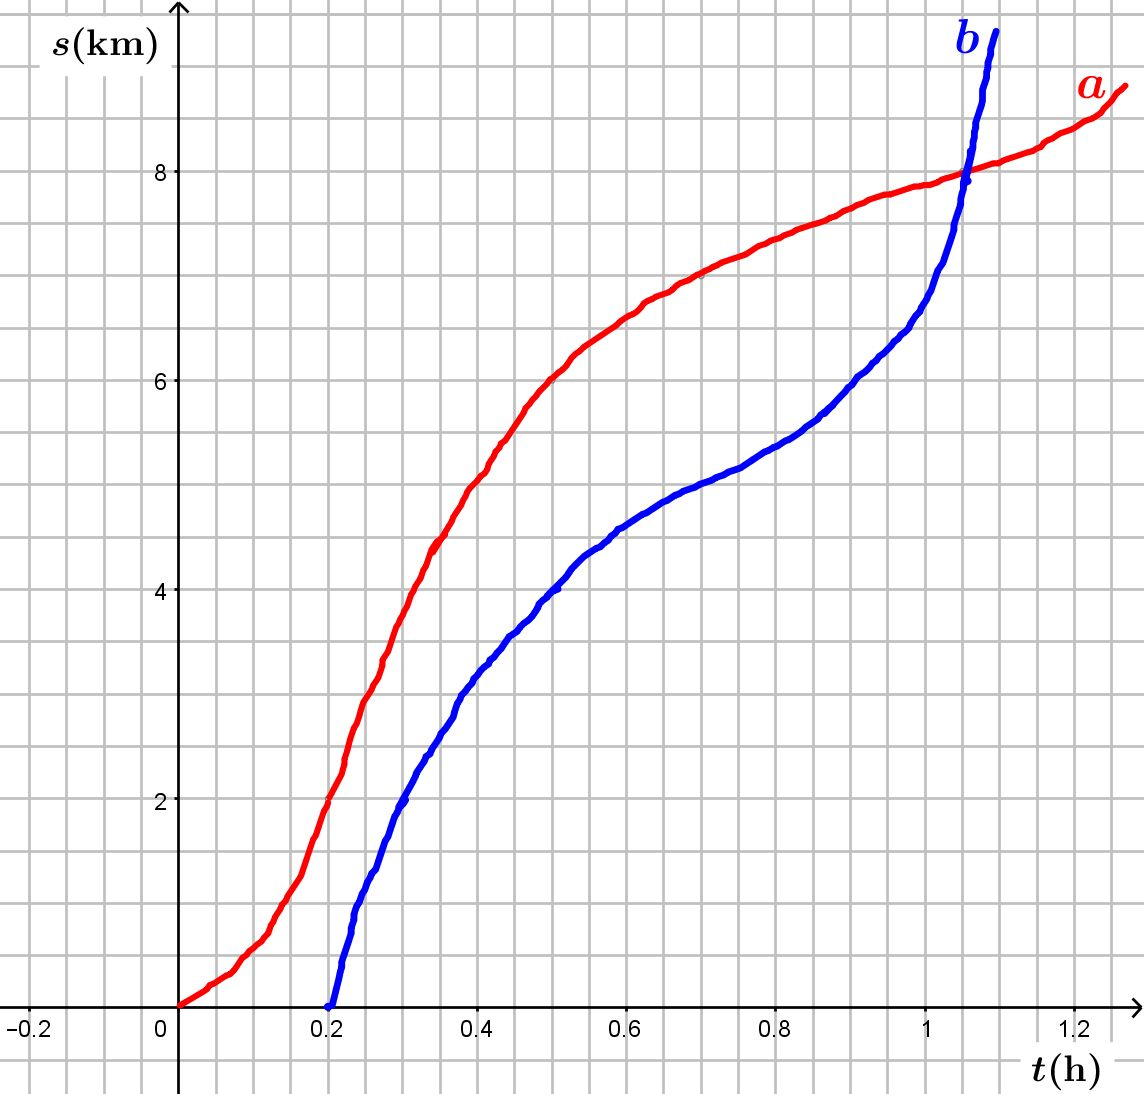
\includegraphics[width=9cm]{img/joggers.jpg}
\end{center}
De beide dames hebben een loophorloge om met GPS-functie. Dat horloge geeft onder andere hun gemiddelde snelheid vanaf het begin aan en ook hun ogenblikkelijke snelheid.
\begin{nummering}
\item Bereken de gemiddelde snelheid van An gedurende het eerste half uur dat zij loopt. Je mag op de grafiek benaderde waarden aflezen.
\item Leg uit hoe je op de grafiek de ogenblikkelijke snelheid van An op het tijdstip $t=0,5$~\textrm{h} kunt aflezen. Lees die snelheid bij benadering af.
\item Op welk moment tijdens haar loop geeft het horloge van Britt de kleinste gemiddelde snelheid aan? Verklaar en duid aan op de grafiek.
\item Op het moment dat Britt An inhaalt, geeft haar horloge een grotere gemiddelde snelheid aan dan dat van An. Leg uit hoe je dat aan de grafiek kunt zien. 
\item Lees vervolgens op de grafiek af wanneer ongeveer tijdens haar loop het horloge van An dezelfde hoge gemiddelde snelheid aangaf.
\end{nummering}

\eindewerktekst

\tussentitel{Oplossing}
\begin{center}
    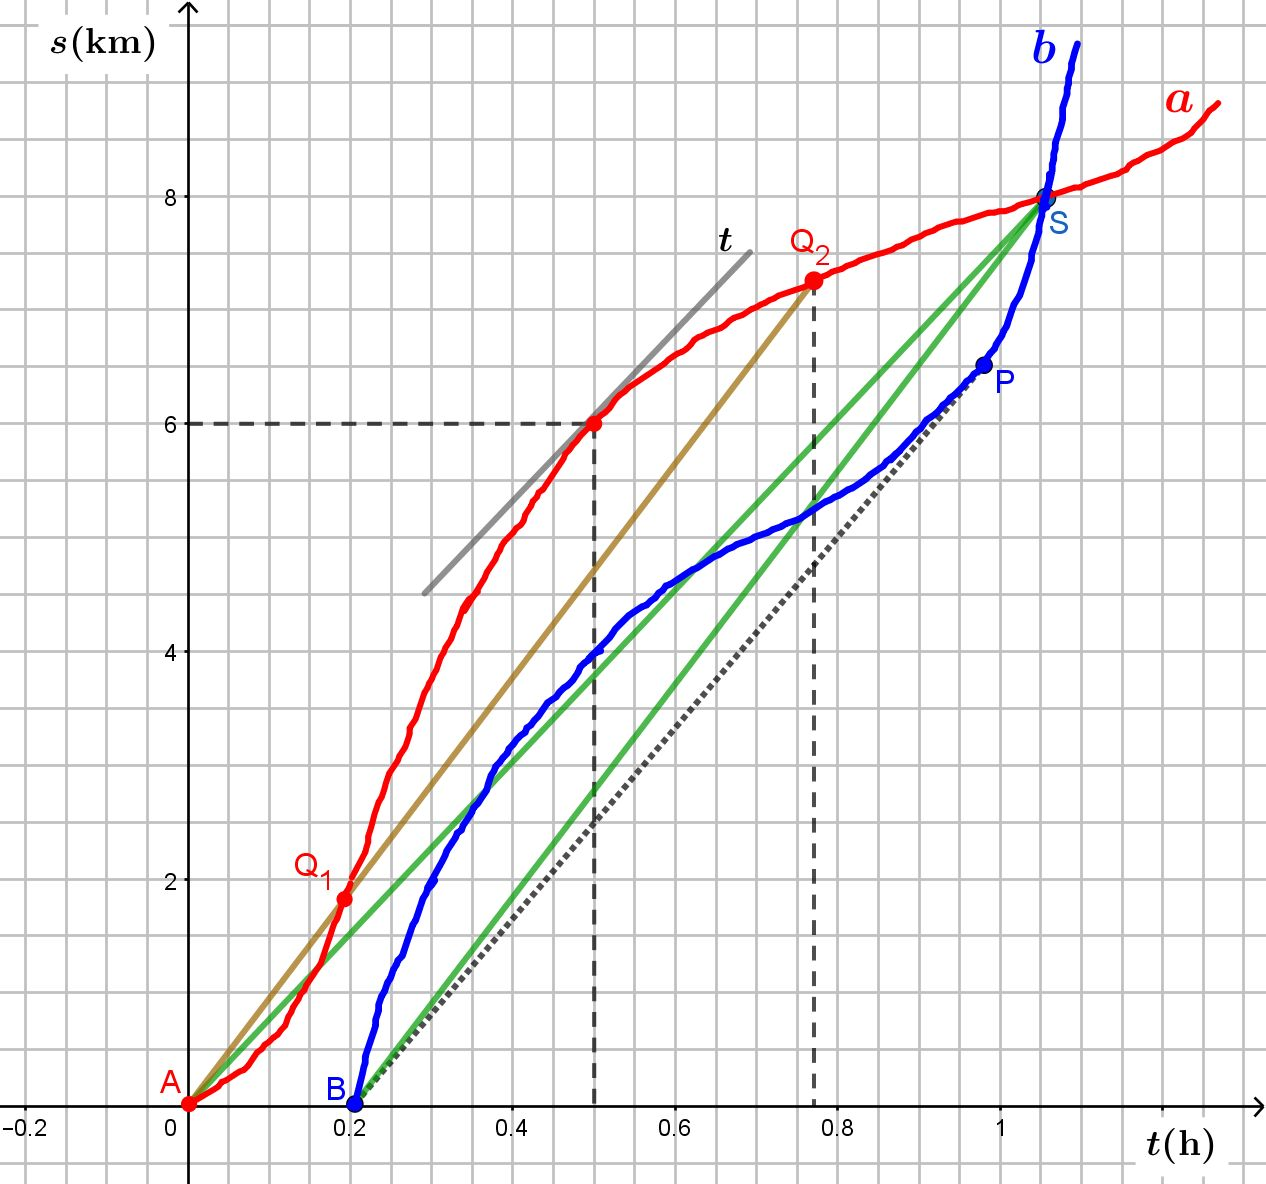
\includegraphics[width=11.7cm]{img/joggers2.jpg}
    %\captionof{figure}{\ }
\end{center}


\begin{nummering}
\item An loopt ongeveer $6$ km in een half uur. Haar gemiddelde snelheid is dus ongeveer $12$ km/h.
\item De ogenblikkelijke snelheid op $t=0,5$\ h is de richtingscoëfficiënt van de raaklijn $t$. Deze is ongeveer gelijk aan $\displaystyle \frac{1,5}{0,2}=7,5$ km/h.  
\item Op $t=0,98$\ h of ongeveer na 59 minuten is de gemiddelde snelheid van Britt het kleinst. De helling van de verbindingslijn $PB$ met het startpunt is daar het kleinst.
\item Je ziet dat de helling van $AS$ kleiner is dan die van $BS$. Op het ogenblik dat Britt An inhaalt, is de gemiddelde snelheid van Britt dus hoger dan die van An.
\item In $Q_1$ en $Q_2$ met  $AQ_i\parallel BS$ is de gemiddelde snelheid van An dezelfde als die van Britt in $S$. Dit is ongeveer bij $t=0,19$\ h (na 11 minuten) en bij $t=0,77$\ h (na 46 minuten).
\end{nummering}

\tussentitel{Wat maakt deze oefening mooi?}
De oefening is vooral interessant omdat ze veel conceptueel inzicht vraagt. In het vierde jaar hebben leerlingen het vaak lastig met het begrip differentiequotiënt. Ze kennen wel de formule voor de richtingscoëfficiënt van een rechte, maar echt conceptueel inzicht in het idee van gemiddelde verandering van een grootheid is moeilijk. Ook het begrip ogenblikkelijke verandering en de link met raaklijnen is niet eenvoudig. De klassikale bespreking van deze oefening is een ideale gelegenheid om het inzicht in deze moeilijke concepten te bevorderen. Bovendien maak je via deze oefening expliciet de transfer naar fysica. De relevantie van wiskunde wordt hier getoond.



\subsection{Ruimtemeetkunde (perspectief) en gelijkvormige driehoeken}
\beginwerktekst{Het tuinpad}

Om een tuinpad een minder klassiek uiterlijk te geven, wil men het betegelen met grote betonnen tegels. Op de afbeelding hieronder is de eerste tegel al gelegd. Zoek uit hoeveel tegels nodig zijn om het hele pad verder te betegelen.\\ Je antwoord moet meer zijn dan een schatting. Zoek een goede argumentering.
\begin{center}
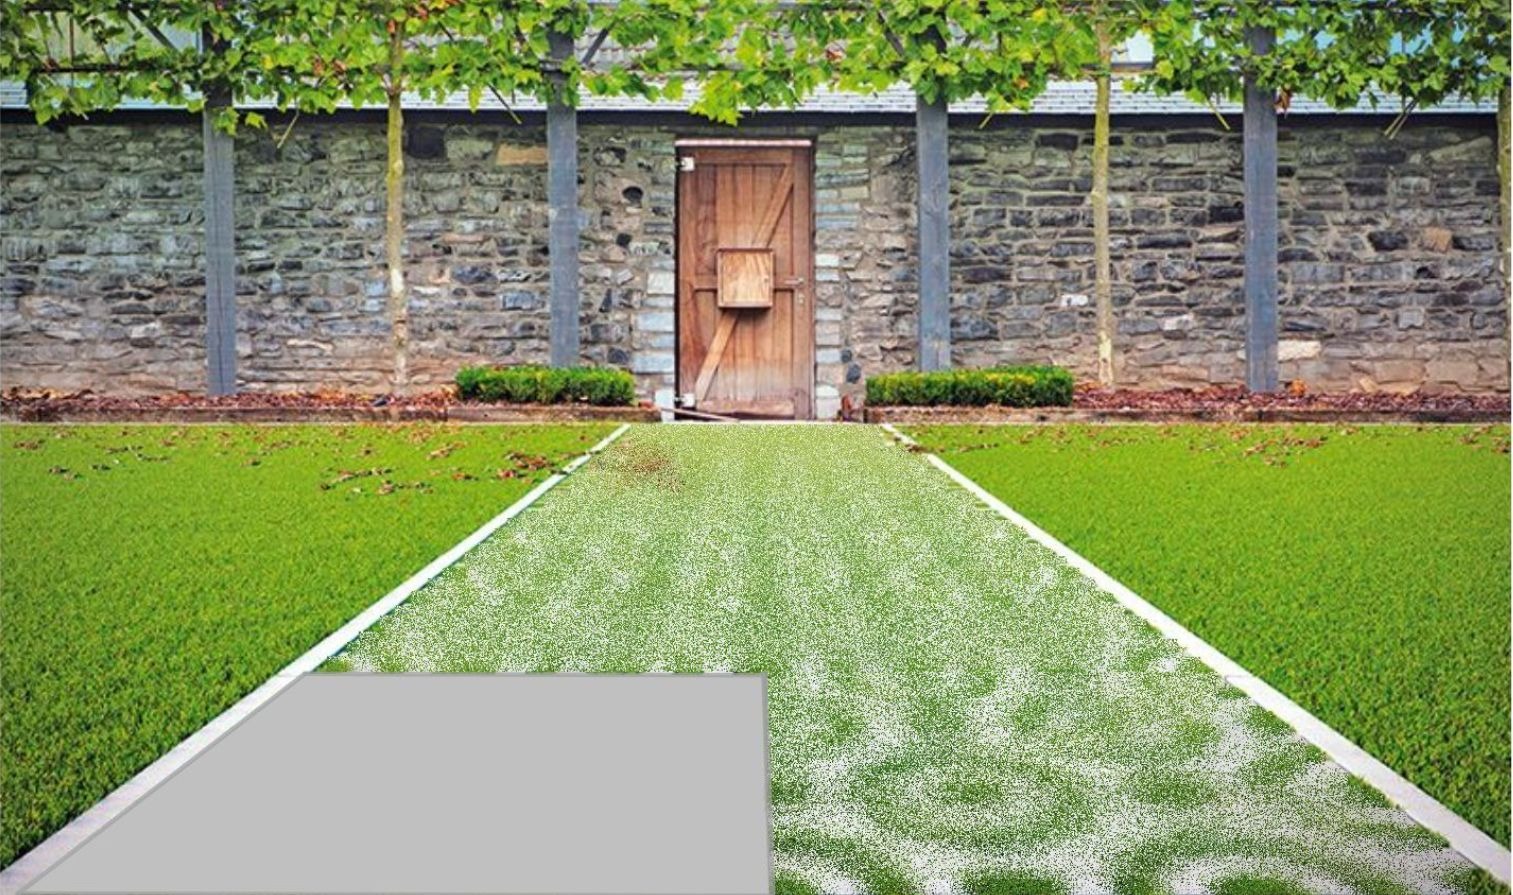
\includegraphics[width=\linewidth]{img/perspectief.jpg}
\end{center}

\eindewerktekst

\tussentitel{Oplossing}
De oplossing kan gevonden worden door opeenvolgende middens te construeren als snijpunten van diagonalen. Dit wordt getoond in onderstaande figuur. Het eerste midden dat je vindt, het midden van het tuinpad, is $M$.  Je ziet dat er net vier tegels passen in een kwart van het pad. Het benodigd aantal tegels is dus 16.
\begin{center}
    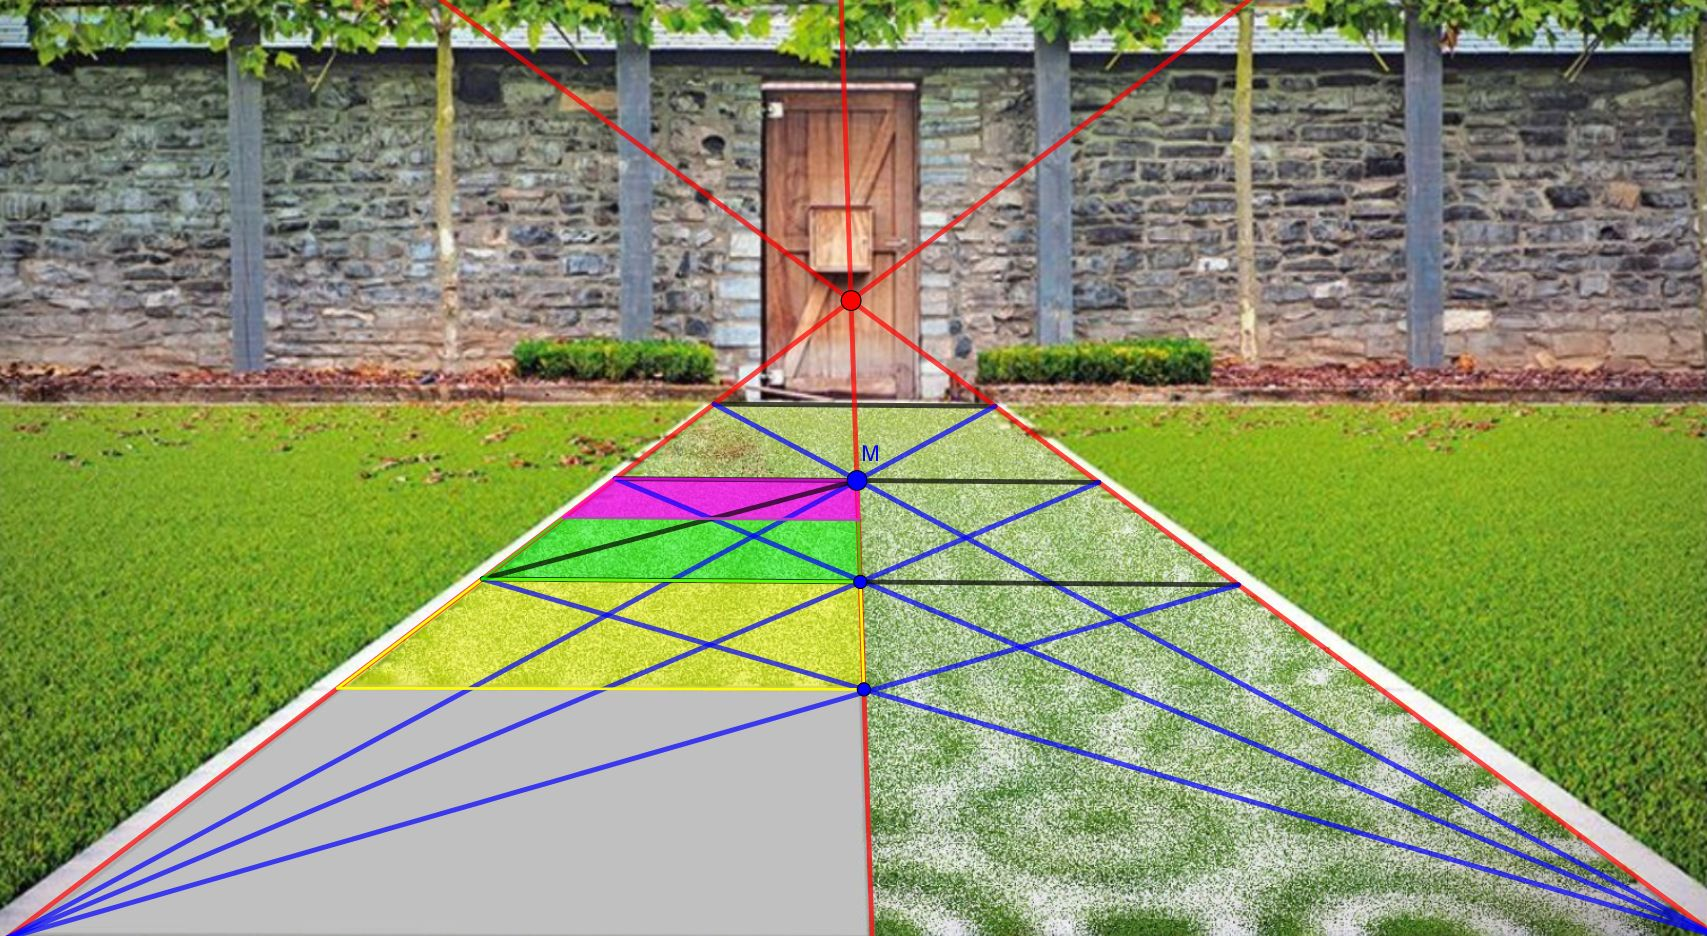
\includegraphics[width=14cm]{img/oplossing_tuinpad.jpg}
    %\captionof{figure}{Een gedeeltelijke betegeling van het tuinpad}
\end{center}
Je kunt dit probleem ook via vluchtpunten oplossen, maar daar komen de meeste leerlingen zelf niet op.

\tussentitel{Wat maakt deze oefening mooi?}
Leerlingen vinden dit een heel leuke oefening omdat ze erg verrast zijn door de perspectivistische vertekening. Vooral de positie van het midden is verrassend. Ze verwachten niet dat het midden \aanh{zo ver weg} ligt. Het is een heel duidelijke illustratie van het feit dat verhoudingen niet bewaard blijven bij centraalperspectief. Leerlingen willen bij het oplossen van dit probleem vaak iets berekenen. Sommigen denken dat de afstanden lineair afnemen. In die context is ook nog volgende oefening interessant.
\begin{center}
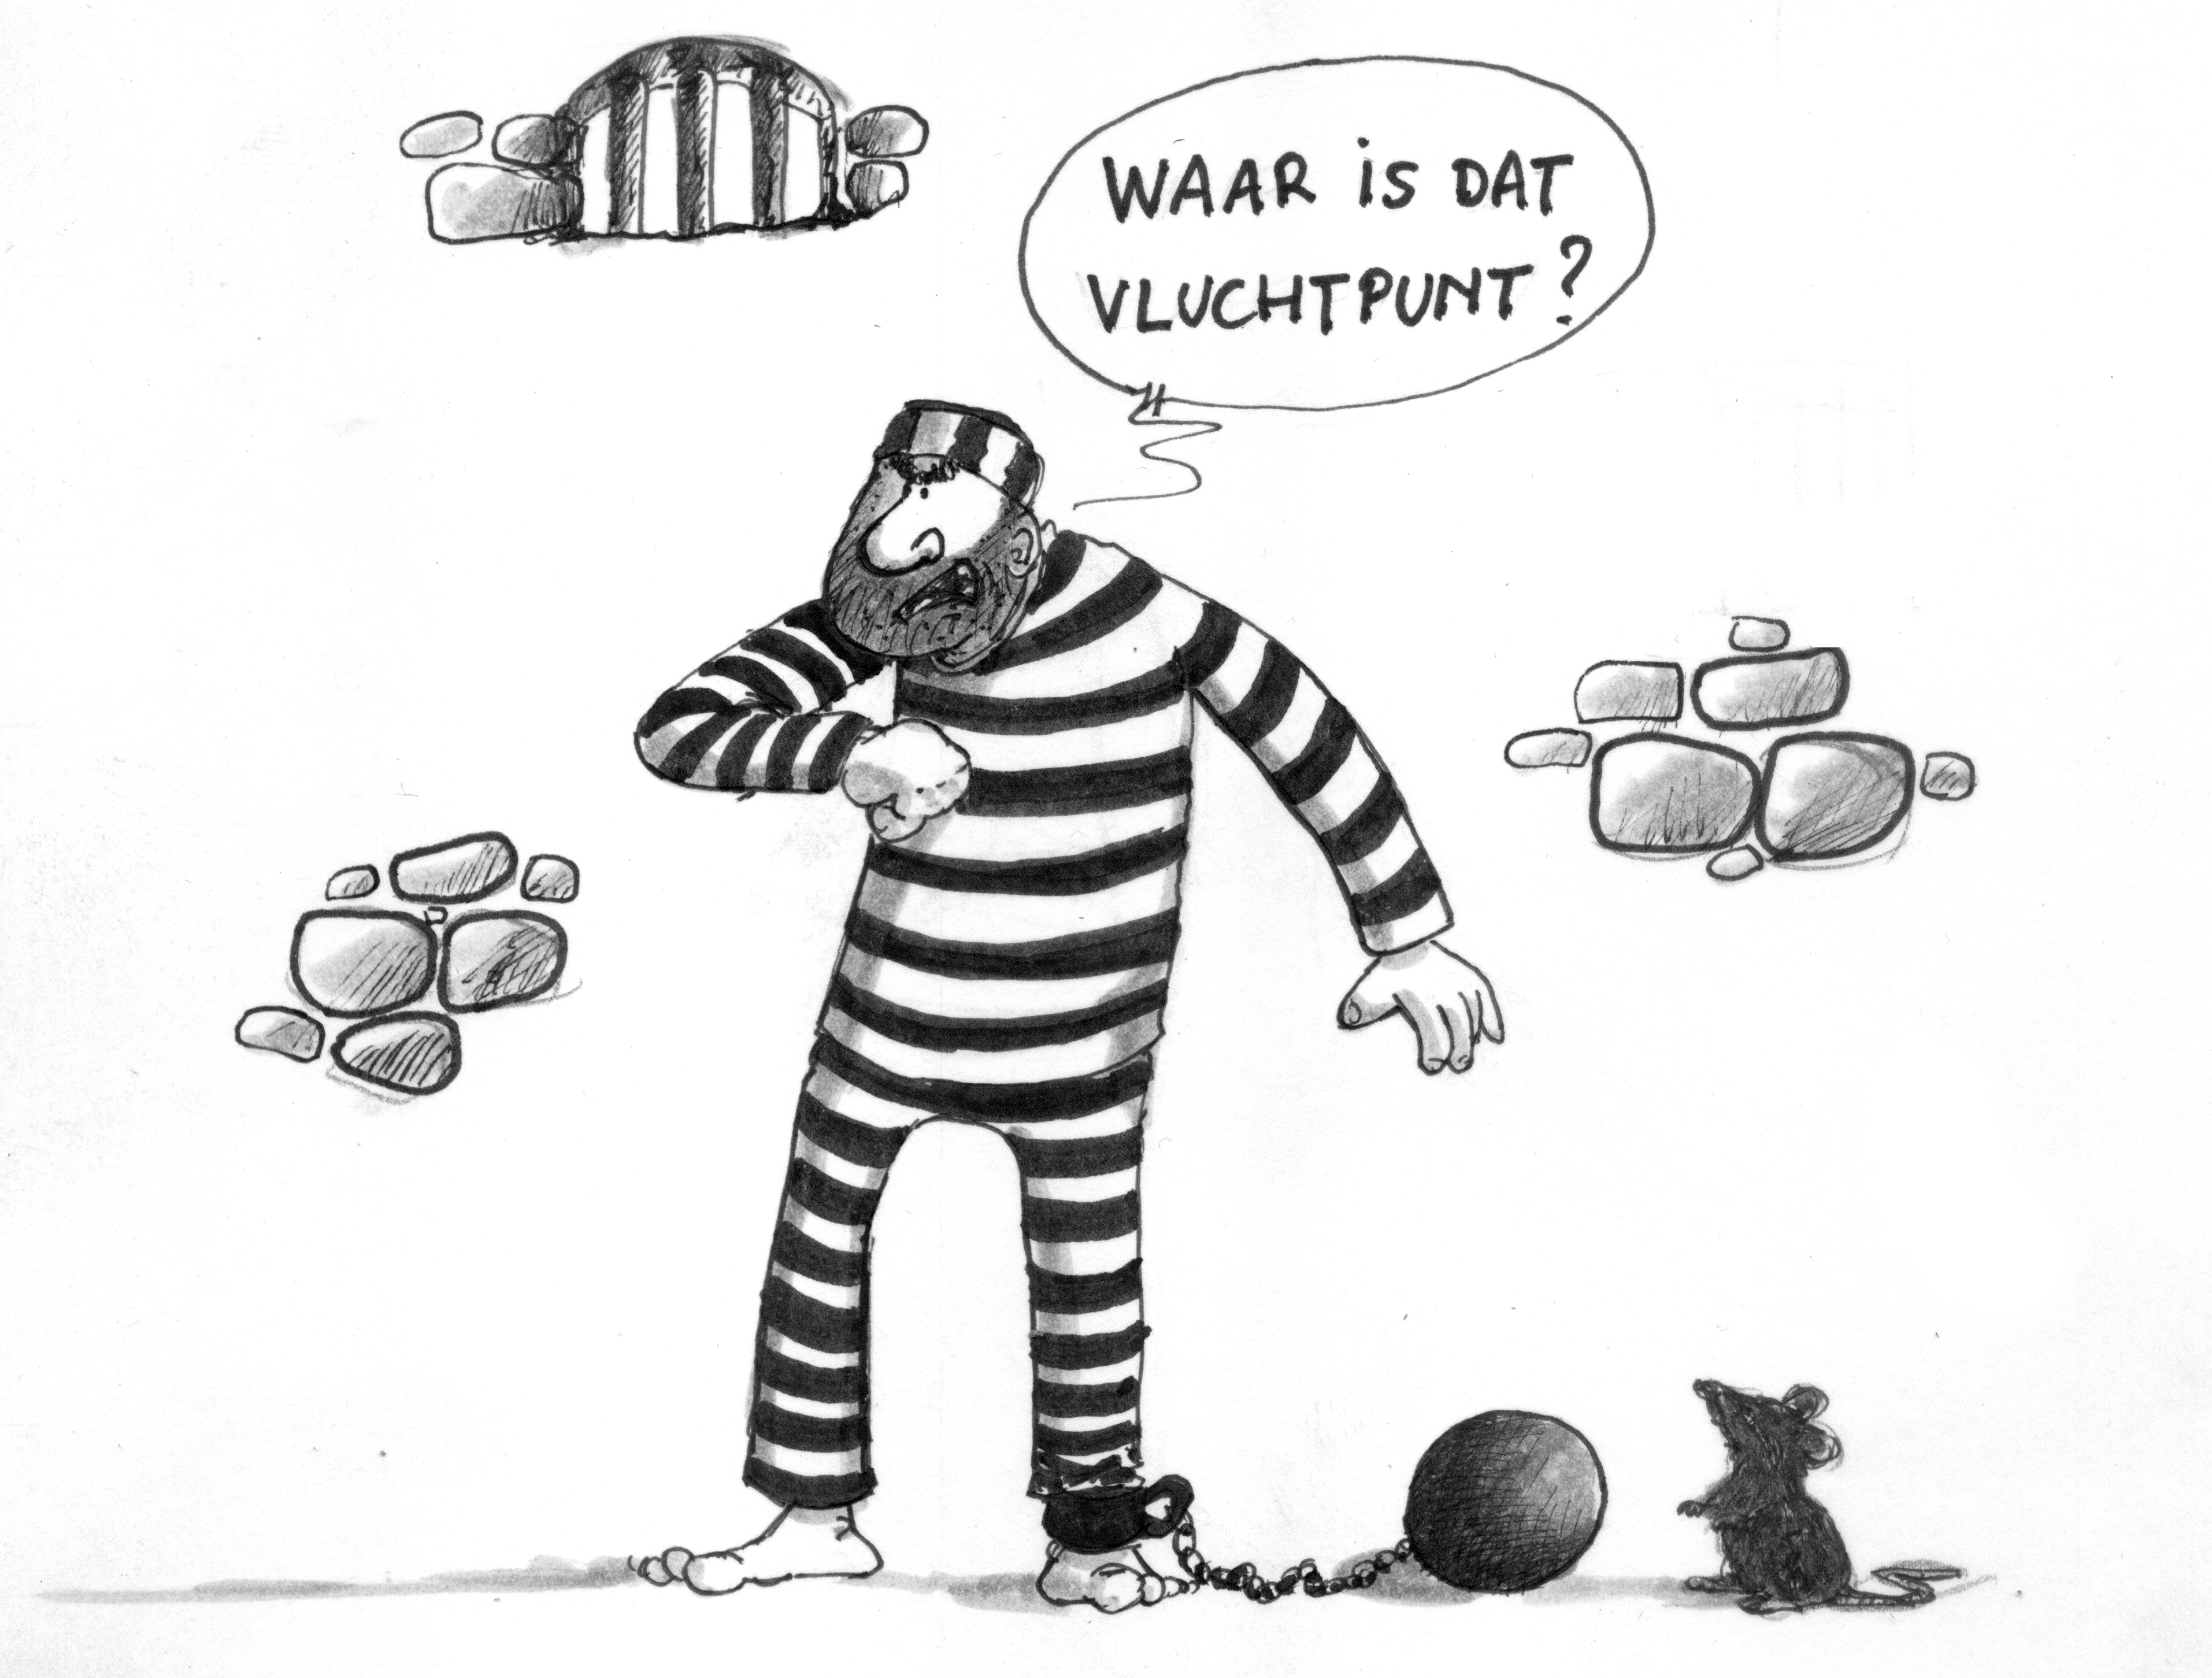
\includegraphics[width=14cm]{img/vluchtpunt.jpg}
\end{center}
\beginwerktekst{Busje rijdt weg}

\figuurrechts{12cm}{2cm}{Tim kijkt door het raam naar buiten en ziet een bestelbusje van hem wegrijden. Het busje rijdt daarbij met een constante snelheid. Tim ziet de achterkant van het busje zoals in de figuur hiernaast. Hij ziet het busje kleiner en kleiner worden.}{\includegraphics[width=1.25cm]{img/perspectief2.png}}

Hieronder staat een zijaanzicht van de situatie.
\begin{center}
\includegraphics[width=9cm]{img/perspectief3.png} 
\end{center}
Op de figuur is aangegeven waar de achterkant van het bestelbusje zich bevindt na 0, 1 en 2 seconden.
\begin{nummering}
	\item Geef op het raam het busje aan zoals Tim dat ziet op de tijdstippen 0, 1 en 2 seconden. Gebruik telkens een andere kleur.
	\item Tim ziet de achterkant van het busje steeds minder hoog. Neemt de hoogte op het raam gedurende de eerste en gedurende de tweede seconde even veel af?
	\item Stel dat de afstand van het oog tot het raam gelijk is aan $k$, dat de afstand van het raam tot het busje gelijk is aan $x$ en dat het busje hoogte $a$ heeft. Bereken dan de hoogte $h$ van het busje op het raam.
	\item Veronderstel dat de weg waarover het busje rijdt lang en recht is, zonder obstakels. Na enige tijd ziet Tim het busje nauwelijks nog: het is niet groter dan een stip. Waar op het raam ziet hij die stip?
\end{nummering}

\eindewerktekst

\tussentitel{Oplossing}
\begin{center}
    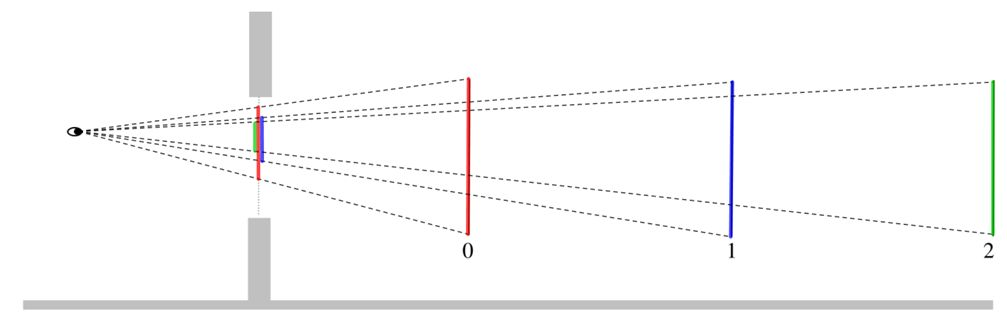
\includegraphics[width=9cm]{img/oplossing_bestelbusje.jpg}
  % \captionof{figure}{Het busje zoals Tim dat ziet op het raam}
\end{center}
\begin{nummering}
    \item In de figuur hierboven zie je de verschillende hoogten van het busje op het raam getekend.
    \item Nee. Je kunt de leerlingen de verschillende hoogten met een meetlat laten meten en een tabel laten maken met de verschillen. Uiteraard hangen de afmetingen af van de schaal waarop je de figuur hebt getekend (druk die zeker voldoende groot af). Je kunt ook een meting met GeoGebra doen. Moest de hoogte telkens even veel afnemen (zoals sommige leerlingen denken), dan zou je uiteindelijk een negatieve hoogte op het raam krijgen. Dat kan natuurlijk niet. 
    \item Dit is een eenvoudige oefening op gelijkvormige driehoeken (zie figuur hieronder). We vinden: $h=\frac{ak}{k+x}$. 
    \begin{center}
    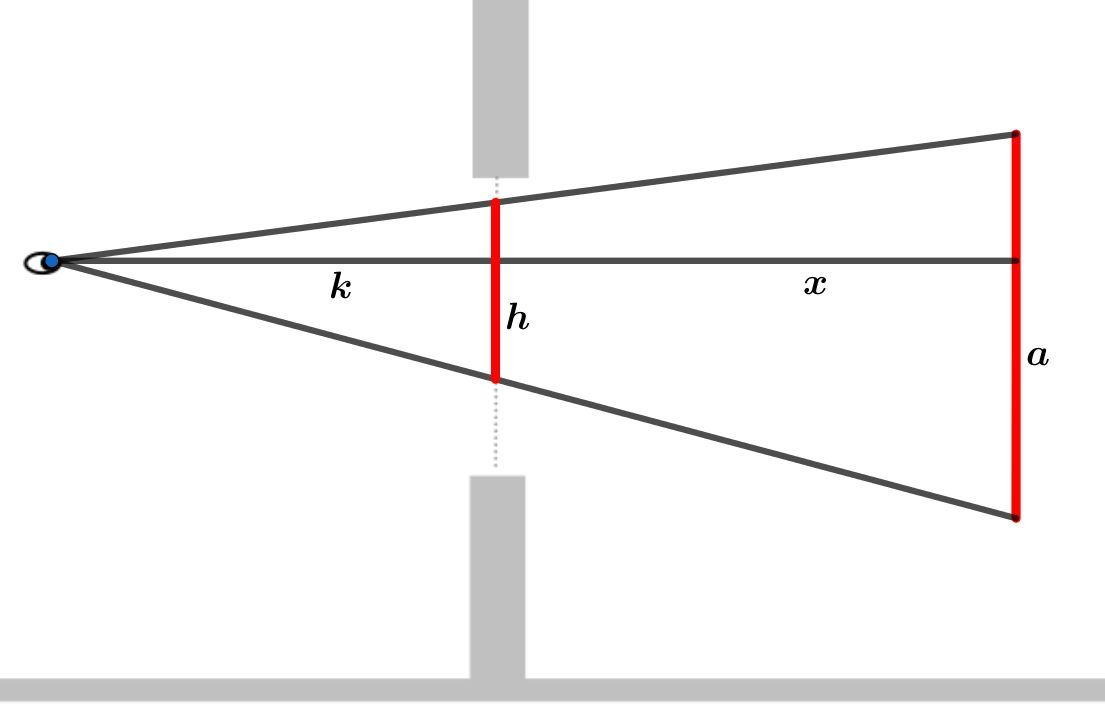
\includegraphics[width=8cm]{img/oplossing_bestelbusje2.jpg}
     \end{center}
    %\captionof{figure}{}
    \item Tim ziet die stip op ooghoogte, recht voor zich. De loodrechte projectie van zijn oog op het raam dus.
 \end{nummering}

\subsection{Oplossen van willekeurige driehoeken}

\beginwerktekst{Een speciaal toeristentreintje}

Op onderstaande figuur zie je een kegelvormige berg met als grondvlak een cirkel. De top staat recht boven het midden. Op de figuur zijn ook de afmetingen gegeven.
\begin{center}
    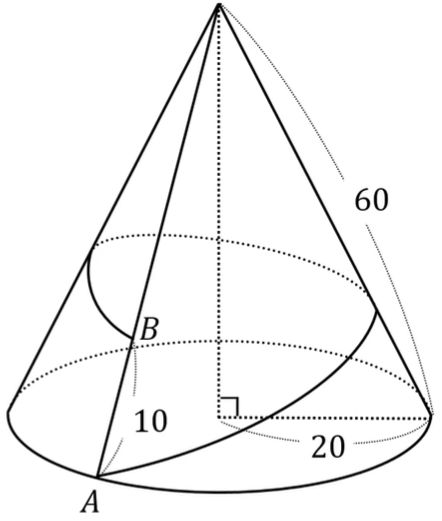
\includegraphics[width=4.5cm]{img/kegel_kortste_pad.jpg}
\end{center}
Voor een toeristentreintje rond de berg moet het kortste pad van punt $A$ naar punt $B$ bepaald worden. Vreemd genoeg blijkt die kortste weg eerst omhoog te lopen en daarna terug te dalen.
\begin{nummering}
\item Bepaal de lengte van het kortste pad langs de kegel van $A$ naar $B$.
\item Wat is de lengte van het dalend stuk?
        \begin{meerkeuze}
            \item $\displaystyle \frac{200}{\sqrt{19}}$
            \item $\displaystyle\frac{300}{\sqrt{30}}$
            \item $\displaystyle\frac{300}{\sqrt{91}}$
            \item $\displaystyle\frac{400}{\sqrt{91}}$
        \end{meerkeuze}
\end{nummering}
\eindewerktekst


\tussentitel{Oplossing}
\begin{nummering}
\item Als je de kegel ontwikkelt in een vlak zoals op de figuur hieronder aangegeven, krijg je een cirkelsector. Je kunt dit door de leerlingen laten doen met een papieren model dat ze open snijden en plat leggen.
\begin{center}
    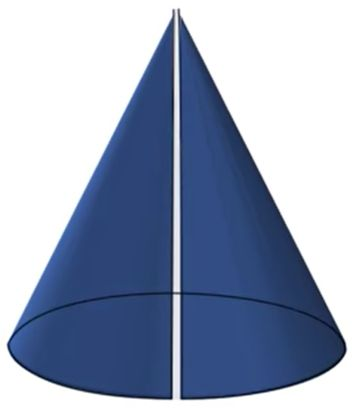
\includegraphics[width=3cm]{img/kegel_kortste_pad2.jpg}\ \ 
    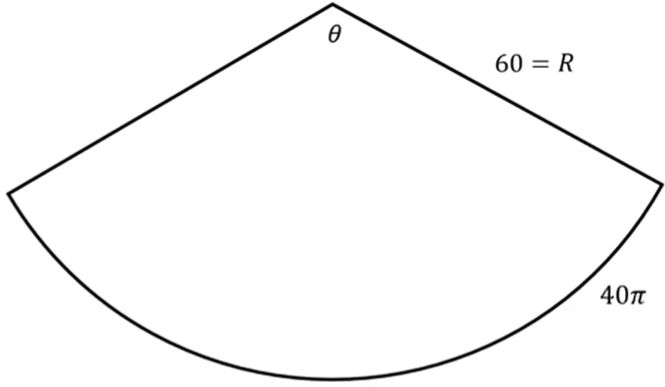
\includegraphics[width=5.75cm]{img/kegel_kortste_pad3.jpg}
    %\captionof{figure}{De ontwikkeling van de kegel}
    \end{center}
De straal van die cirkelsector is 60. De lengte van de cirkelboog is de omtrek van het grondvlak van de kegel (een cirkel met straal $r=20$): $2\pi r=40\pi$.
Hiermee kunnen we de middelpuntshoek $\theta$ berekenen. Een hele cirkel met straal 60 heeft een omtrek van $120\pi$. De booglengte $40\pi$ is hier net een derde deel van. De middelpuntshoek moet dus ook een derde deel zijn van $360^\circ$. Dus: $\theta=120^\circ$.\\
We duiden nu de punten $A$ en $B$ op de cirkelsector aan en bepalen de kortste weg van $A$ naar $B$: een rechte lijn. Met de cosinusregel kun je daarvan de lengte berekenen. We vinden: $$|AB|=10\sqrt{91}.$$
\begin{center}
       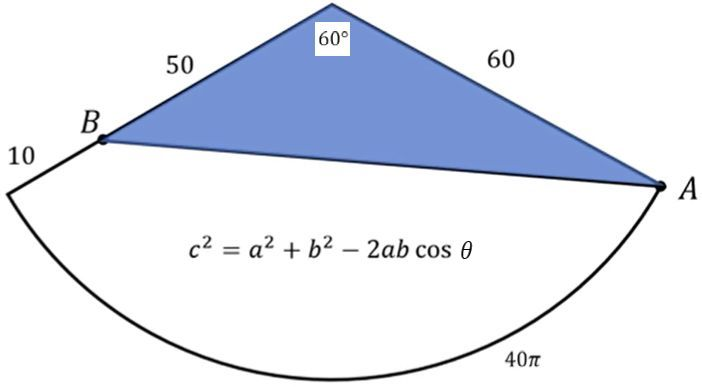
\includegraphics[width=7cm]{img/kegel_kortste_pad4.jpg}
%    \captionof{figure}{Het kortste pad met de cosinusregel}
\end{center}
\item Er is gegeven dat er een stijgend stuk en een dalend stuk is in het kortste pad. Je kunt dit als volgt inzien. Bij de gepunte lijnen rechts van het lijnstuk $[T,U]$, zoals bijvoorbeeld $[T,W]$ nemen de afstanden van een punt $X$ op het pad tot de top $T$ van de kegel af wanneer je vertrekt in $A$. De afstand $|XW|$ tot de \aanh{grond} (langsheen het oppervlak van de kegel) neemt daar dus toe. De kortste afstand van een punt van het pad tot de top $T$ vinden we in $V$ waarbij $TV\perp AB$. Vanaf het punt $V$ begint de afstand van een punt van het pad (bijvoorbeeld $Z$) tot de top $T$ weer toe te nemen. Bijgevolg nemen de afstanden $|YZ|$ af. Vanaf $V$ begint dus het pad te dalen.   

\begin{center}
       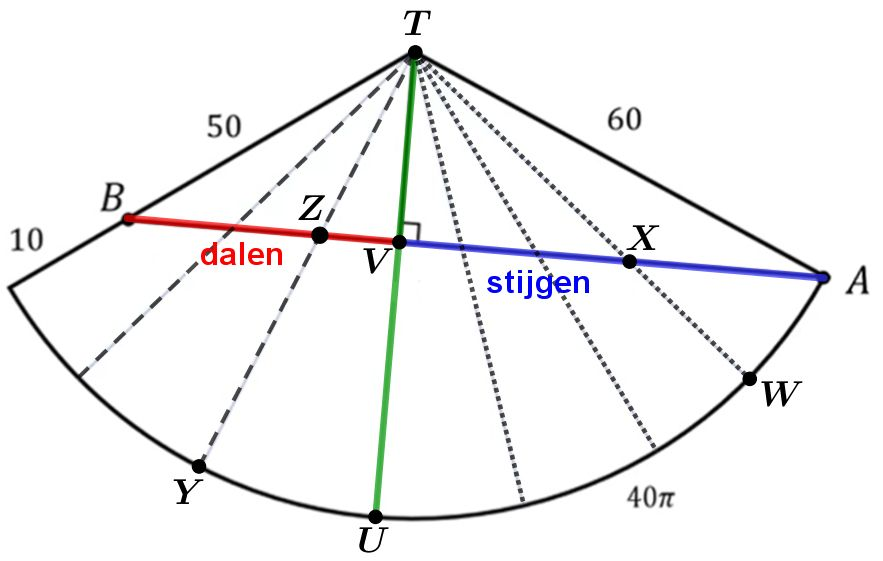
\includegraphics[width=9cm]{img/kegel_kortste_pad5.jpg}
   % \captionof{figure}{Stijgen en dalen}
\end{center}

Om nu de lengte van het dalende stuk te berekenen, gebruiken we de stelling van Pythagoras. Met de letters zoals in onderstaande figuur geldt:
\begin{align*}
    (10\sqrt{91}-x)^2+h^2 &= 60^2\\
    x^2+h^2 &=50^2
\end{align*}

Als we de twee bovenstaande vergelijkingen lid aan lid van mekaar aftrekken, vinden we na enig rekenwerk $$x=\frac{400}{\sqrt{91}}.$$


\begin{center}
       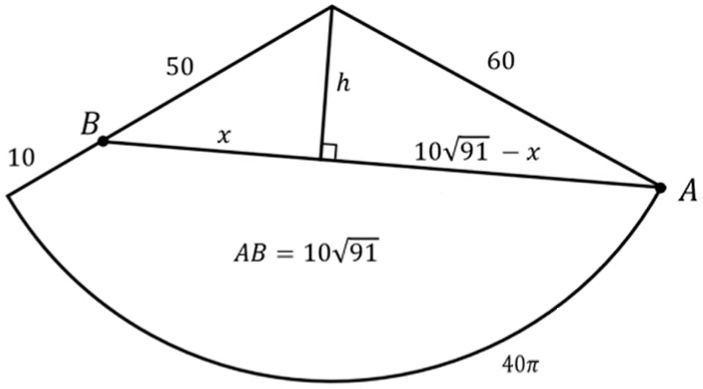
\includegraphics[width=9cm]{img/kegel_kortste_pad6.jpg}
   % \captionof{figure}{Lengte van het dalende stuk}
\end{center}
\end{nummering}

\tussentitel{Wat maakt deze oefening mooi?}
De context van de berg en het treintje is bij de haren getrokken, maar verder is dit een oefening die best wel origineel is en goed gebruikt kan worden om te differentiëren. Je zult in de les wellicht een tip moeten geven door de leerlingen een papieren model van de kegel en een schaar te geven. Sterke leerlingen kun je beide vragen laten beantwoorden, leerlingen die zwakker zijn in wiskunde zullen al een hele kluif hebben aan oefening 1. Mooi aan deze oefening is ook dat ze verwondering opwekt. De meeste leerlingen verwachten dat je steeds moet stijgen om volgens de kortste weg van $A$ naar $B$ te gaan.\\ Een bijkomende vraag, misschien voor een onderzoek door leerlingen, kan zijn of het bij alle kegelvormige bergen zo is dat er een dalend stuk is.





\section{Derde graad}

\subsection{Raaklijnen aan de grafiek van de sinusfunctie}

\beginwerktekst{Een raaklijn aan de grafiek van de sinusfunctie}

Geef een vergelijking van een rechte die door de oorsprong gaat en in juist twee punten raakt aan de grafiek van $x \mapsto \sin x$.\\
Maak een schets. 
Hoeveel oplossingen heeft het probleem volgens jou? 

\eindewerktekst

\tussentitel{Oplossing}

We maken een schets. Na wat proberen (bijvoorbeeld met GeoGebra) vinden we de volgende oplossing. 

\begin{center}
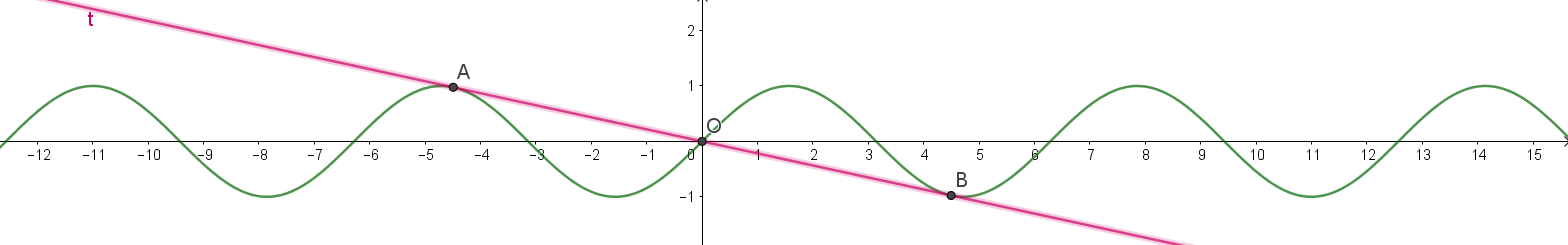
\includegraphics[width=\linewidth]{img/sinus1.jpg}
%\captionof{figure}{}
\end{center}


Nog wat verder experimenteren leert ons dat er meer oplossingen zijn; er zijn er zelfs oneindig veel!

\begin{center}
\includegraphics[width=\linewidth]{img/sinus2.png}
%\captionof{figure}{}
\end{center}


We geven hieronder twee manieren om deze opgave op te lossen. 

\tussentitel{Eerste werkwijze}
De gezochte raaklijn moet door de oorsprong gaan en heeft dus een vergelijking van de vorm $y=mx$.
Het getal $m$ moet de richtingscoëfficiënt van de raaklijn zijn in een punt $B(a,\sin a)$ van de grafiek, dus 

\[m= \cos a .\]

Anderzijds is $m$ ook de richtingscoëfficiënt van de rechte $OB$ (zie figuur). Dus
\[m=\frac{\sin a}{a}.\]
Gelijkstellen geeft:
\[ \cos a = \frac{\sin a}{a}.\]

Of nog:

\[a=\tan a  \text{  en  }  a\neq 0 . \]

Dit is een vergelijking in $a$ die enkel grafisch (of numeriek) kan worden opgelost. Hieronder doen we dat door de nulpunten te bepalen van de functie $x \mapsto x -\tan x $ 

\begin{center}
\includegraphics[width=\linewidth]{img/sinus3.png}
%\captionof{figure}{}
\end{center}

Deze functie is oneven, zodat de nulpuntenverzameling symmetrisch is rond 0. We kunnen ons beperken tot de positieve oplossingen $4,49; 7,73;\cdots $ (Merk op dat die geen rekenkundige rij vormen! Leg grafisch uit.) Omdat de sinusgrafiek puntsymmetrisch is ten opzichte van de oorsprong, is het telkens dezelfde raaklijn die raakt in $(a, \sin a)$ en in $(-a,\sin (-a)) $. De gevraagde raaklijnen zijn dan 
\begin{align*}
    y &= x \cos (4,49)\\
    y &= x \cos (7,73)\\
    \cdots
\end{align*}
Er zijn oneindig veel oplossingen. Er is een oplossing waarbij de raaklijn de grafiek behalve in twee punten raakt, de sinusgrafiek ook nog in 1 punt snijdt ($y=x \cos (4,49)$) of in 3 punten ($y=x \cos (7,73)$), of in 5 punten, enz. (algemeen: er is bij elk oneven aantal snijpunten een raaklijn te vinden). Dit vormt een mooi tegenvoorbeeld voor de misvatting dat een raaklijn de kromme maar in één punt ontmoet.

De figuur hieronder illustreert dat de raakpunten niet periodiek zijn. Indien die wel periodiek zouden zijn, zouden al die raaklijnen dezelfde richtingsco\"effici\"ent hebben, wat uiteraard niet kan.

\begin{center}
\includegraphics[width=\linewidth]{img/sinus4.png}
%\captionof{figure}{}
\end{center}


\tussentitel{Tweede werkwijze}

Je kunt ook vertrekken van een willekeurige raaklijn aan de grafiek en dan eisen dat de oorsprong op deze rechte ligt. De raaklijn in het punt $B(a,\sin a)$ heeft als vergelijking
\[y-\sin a = \cos a \cdot (x-a).\]
De oorsprong ligt op deze rechte indien $-\sin a = \cos a \cdot (-a) $). Dit kunnen we herschrijven tot de vergelijking 
\[a=\tan a .\]
Vanaf hier verloopt deze oplossingswijze zoals hierboven beschreven.

\tussentitel{Wat maakt deze oefening mooi?}

Aanvankelijk denken sommige leerlingen dat de gezochte raaklijn de sinusgrafiek raakt in een top. Dit kan uiteraard niet, want de raaklijnen in de top zijn horizontaal en gaan dus niet door de oorsprong.

De gevonden raaklijn snijdt de grafiek ook elders. Leerlingen hebben nood aan dergelijke voorbeelden om hen van hun misverstanden hierover af te helpen.

Ten slotte is er ook nog het verrassende van de oneindig veel oplossingen, maar wel \textit{zonder} periodiciteit. Bij goniometrische functies lijkt periodiciteit te horen zoals Nicole bij Hugo.

Bij de eerste werkwijze komen twee visies op ‘richtingsco\"effici\"ent’ bij elkaar (richtingsco\"effici\"ent van een rechte bepaald door twee punten en de afgeleide als richtingscoëfficiënt van de raaklijn). Dit is hier de sleutel tot de oplossing. Bij de tweede werkwijze gaat het over een goed begrip van de betekenis van een vergelijking van een rechte.

Verder bots je ook nog op een transcendente vergelijking. Door de handboekoefeningen krijgen leerlingen soms ten onrechte de indruk dat in wiskunde alles \aanh{mooi uitkomt} ...

De berekeningen blijven al bij al redelijk eenvoudig. 

\subsection{Een verrassende afgeleide}

\beginwerktekst{Een eenvoudige oefening?}

Bereken $ \frac{\mathrm{d}}{\mathrm{d}x} \arcsin (\sin x)$.

\eindewerktekst

\tussentitel{Oplossing}

De meeste leerlingen beginnen meteen te rekenen. Dit is niet verwonderlijk; de oefening staat in een reeks en bij alle vorige oefeningen moest je gewoon beginnen afleiden. Zij vinden:

\begin{align*}
    \frac{\mathrm{d}}{\mathrm{d}x} \arcsin (\sin x) &= \frac{1}{\sqrt{1-\sin^2 x}}\cdot \cos x \\
    &= \frac{1}{\cos x} \cdot \cos x \\
    &= 1
\end{align*}

Tijdens deze berekening vraagt een leerling \aanh{moet het niet plus of min de wortel zijn}? Een andere leerling antwoordt: \aanh{Neen, want een $\mathrm{arcsinus}$ is altijd in $[-\frac{\pi}{2},\frac{\pi}{2}]$ en de cosinus is daar positief}. De klas keurt dit goed, ook al begrijpen ze het niet helemaal. De leerling die sprak heeft immers  een goede wiskundereputatie.
Andere leerlingen \aanh{kijken} voor ze beginnen te rekenen. Ze zeggen dat \aanh{inverse functies elkaar opheffen} en doen dit zo:
\[\frac{\mathrm{d}}{\mathrm{d}x} \arcsin (\sin x) =  \frac{\mathrm{d}}{\mathrm{d}x} x = 1 .\]
Iedereen vindt hetzelfde resultaat. Dat moet dan toch kloppen, niet? Ik laat het grafisch controleren. De grafiek van de af te leiden functie maakt duidelijk dat er iets mis is met de oplossing.
\begin{center}
\includegraphics[width=0.6\linewidth]{img/arcsin1.png}
%\captionof{figure}{}
\end{center}
De afgeleide is blijkbaar niet \aanh{overal} gelijk aan 1: in sommige intervallen wel en in andere intervallen is die gelijk aan $-1$.
Wat was er dan fout aan de uitleg over de cosinus die in dat interval positief is? En heffen de sinus en de arcsinus elkaar niet op?
We komen erachter dat $x\mapsto \arcsin (\sin x) $ niet zomaar $x$ kan zijn: $x$ kan gelijk welke waarde in $\R$ aannemen, $\sin x$ is een element van $[-1,1]$ en de arcsinus hiervan is een element van $[-\frac{\pi}{2},\frac{\pi}{2}]$; als $x$ niet in dat interval zit is $\arcsin (\sin x)$ dus niet gelijk aan $x$. We merken verder ook op dat de functie $x\mapsto \arcsin (\sin x) $ periodiek is met periode $2\pi$. Als we de functie kunnen beschrijven in het interval $[-\frac{\pi}{2},\frac{3\pi}{2}]$, dan weten we precies hoe ze eruitziet. Voor het eerste stuk van dit interval is er geen probleem: als $x \in [-\frac{\pi}{2},\frac{\pi}{2}]$ is $\arcsin (\sin x) = x$. Voor $x \in [\frac{\pi}{2},\frac{3\pi}{2}]$ bekijken we de situatie op de goniometrische cirkel.
\begin{center}
\includegraphics[width=6cm]{img/arcsin2.png}
%\captionof{figure}{}
\end{center}


Omdat supplementaire hoeken gelijke sinussen hebben en omdat $\pi - x$ wel in het juiste interval ligt, is $\arcsin (\sin x)= \pi - x$ indien $x \in [\frac{\pi}{2},\frac{3\pi}{2}]$. Samen met de periodiciteit kunnen we nu de grafiek van $x\mapsto \arcsin (\sin x) $ begrijpen.

Terug naar de eerste berekening. Vermits $x$ gelijk welk reëel getal kan zijn, kan $\cos x$ zowel positief als negatief zijn. De opmerking van de leerling i.v.m. het interval voor arcsin is dus naast de kwestie. Om de uitdrukking correct te vereenvoudigen moeten we absolute-waardetekens gebruiken:

\begin{align*}
    \frac{\mathrm{d}}{\mathrm{d}x} \arcsin (\sin x) &= \frac{1}{\sqrt{1-\sin^2 x}}\cdot \cos x =\frac{\cos x}{\sqrt{\cos^2 x}}= \frac{\cos x}{\lvert{\cos x}\rvert}.
\end{align*}

We kunnen dit zo laten staan, of als een meervoudig voorschrift voorstellen:
\begin{align*}
    \cdots &= \left\{ \begin{array}{ll}
         1 & (\text{als } \cos x > 0)\\
        -1 & (\text{als } \cos x < 0)\end{array} \right.\\
          &= \left\{ \begin{array}{ll}
         1 & (\text{als } x \in ]-\frac{\pi}{2} + 2k\pi, \frac{\pi}{2}+2k\pi[, \quad k \in \Z )\\
        -1 & (\text{als } x \in ]\frac{\pi}{2} + 2k\pi, \frac{3\pi}{2}+2k\pi[, \quad k \in \Z ).\end{array} \right.
\end{align*}\\

Dit is niet korter. Eventueel kan hier de signumfunctie ingevoerd worden om dit compact te noteren. Dan krijgen we 

\[\frac{\mathrm{d}}{\mathrm{d}x} \arcsin (\sin x) =  \text{sgn} (\cos x) .\]

\tussentitel{Wat maakt deze oefening mooi?}

Wat ogenschijnlijk een eenvoudige oefening op afgeleiden was, blijkt toch een heel verrassend kantje te hebben. Door de grafiek van de functie te bekijken konden we niet anders dan onze oplossing in vraag te stellen. Zo zat er meer in deze opgave dan eerst gedacht. Ook over wat er gebeurt in de knikpunten valt er wat te zeggen, maar dat hebben we hier niet uitgewerkt.



\subsection{Rakende grafieken van een exponenti\"ele en een logaritmische functie}

\beginwerktekst{Kussende krommen}

In de figuur hieronder zie je de grafieken van de functies $f(x)=a^x$ en $g(x)= \; ^a \log x$. Deze functies zijn, zoals geweten, elkaars inverse. Bepaal nu het grondtal $a$ waarvoor deze functies aan elkaar raken zoals op de figuur. Bepaal ook de coördinaten van het raakpunt $P$. Zowel voor het grondtal $a$ als voor de coördinaten van $P$ moet je exacte uitdrukkingen geven.

Hint: denk na over de volgende vraag: welke rechte moet die gemeenschappelijke raaklijn zijn?
\begin{center}
\includegraphics[width=10cm]{img/kussen1.png}
\end{center}
\eindewerktekst
\begin{center}
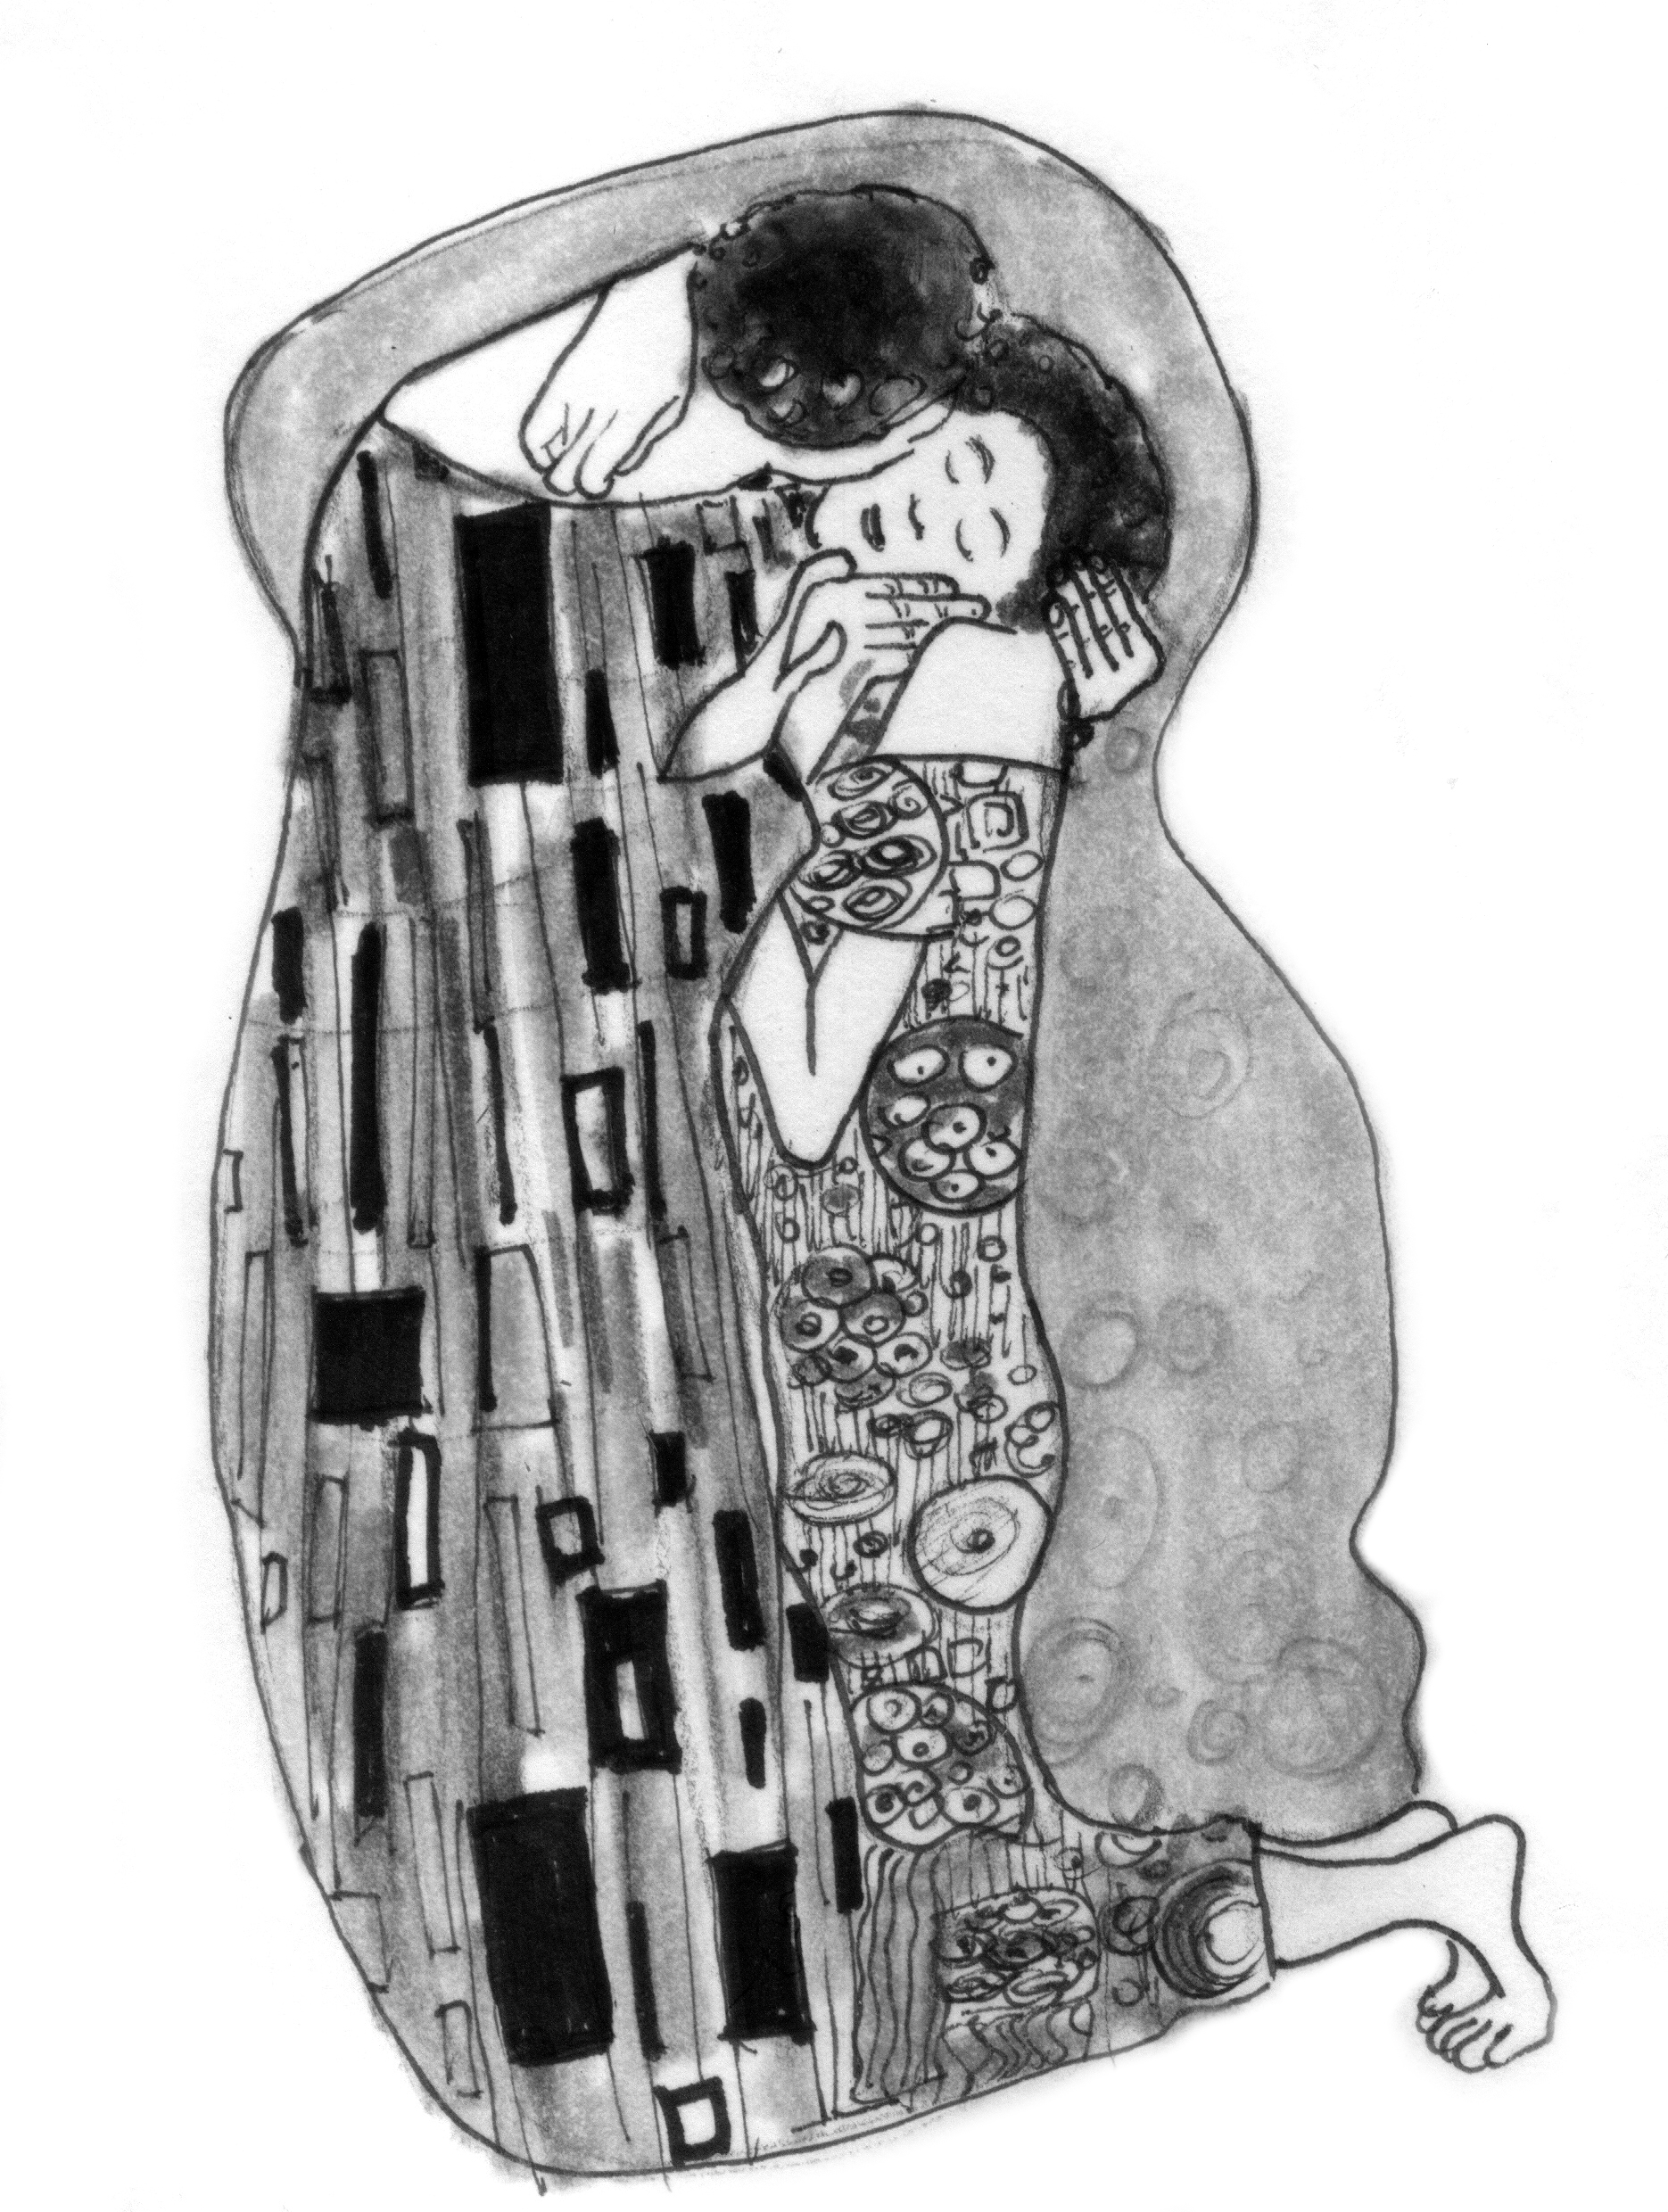
\includegraphics[width=8cm]{img/kus.jpg}
\end{center}

\tussentitel{Oplossing}

Omdat de twee functies elkaars inverse zijn, zijn de grafieken elkaars spiegelbeeld t.o.v. de rechte $y=x$. Het raken van beide krommen moet bijgevolg gebeuren in een punt van deze spiegelas en de raaklijn in dat punt moet de spiegelas zelf zijn. Indien dit niet zo was, dan zouden er in dat punt twee raaklijnen zijn, wat uiteraard niet kan.
We zoeken dus een punt $P(x_0,x_0)$ op de grafiek van $f$ (of die van $g$) waarvoor $f'(x_0)=g'(x_0)=1$. Dit geeft het stelsel

\[ \left\{ \begin{array}{l}
         x_0 = a^{x_0}\\
        \frac{1}{\ln a \cdot x_0} = 1\end{array}. \right. \] 

De eerste vergelijking kunnen we herschrijven als $x_0 = e^{x_0  \ln a}$. De exponent uit deze uitdrukking is 1 zoals we leren uit de tweede vergelijking van het stelsel. Zo vinden we al heel snel $x_0=e.$\\
Door dit in te vullen in één van beide vergelijkingen kunnen we $a$ berekenen, namelijk $a=e^{\frac{1}{e}}$. We zochten dus het punt $P(e,e)$ en het grondtal $a=e^{\frac{1}{e}}$. 

\tussentitel{Wat maakt deze oefening mooi?}

Hoewel de vraagstelling eenvoudig is, is de oplossing dit niet. Een sterke groep zou je de opgave kunnen voorleggen zonder de hint, maar de ervaring leert mij dat slechts weinig leerlingen dan tot een oplossing komen. Je kunt dit wat bespoedigen door de leerlingen eerst wat te laten experimenteren met GeoGebra. De leerlingen kunnen hier zelf een dynamische figuur voor maken (met een schuifbalkje voor $a$). Via de link uit Arnold (2018) kom je bij een kant en klare GeoGebra-applet. Bij de start van het applet ($a=3$) is er nog ruim plaats tussen de twee grafieken. Een eerste ori\"enterend vraagje kan zijn: hoe moeten we $a$ veranderen om de krommen dichter naar elkaar toe te laten komen? Een beetje spelen met het applet laat zien dat er inderdaad een waarde voor $a$ is waarvoor de twee krommen raken. 



\begin{center}
\includegraphics[width=0.49\linewidth]{img/kussen2bijgesnedenzw.png}\ 
\includegraphics[width=0.50\linewidth]{img/kussen3bijgesnedenzw.png}

\end{center}




De opgave doorbreekt de aangeleerde oplossingsstrategie van \aanh{raken betekent zelfde functiewaarde en gelijke afgeleiden}. Deze strategie leidt tot het stelsel

\[ \left\{ \begin{array}{l}
         a^{x_0} = \; ^a \log x_0\\
        \ln a \cdot a^{x_0} = \frac{1}{\ln a \cdot x_0} \end{array}. \right. \] 

Dit stelsel is heel wat lastiger om op te lossen!
Door eerst na te denken over de raaklijn kan het stelsel vervangen worden door één met minder ingewikkelde vergelijkingen, maar toch blijkt dat het vinden van de oplossing voor veel leerlingen niet zo voor de hand te liggen. Wie goed kijkt naar de vergelijkingen en begrijpt wat er staat, zal echter wel snel tot de oplossing komen. 
Wat ook mooi is, is dat het gezochte grondtal geen voor de hand liggende waarde is. Een leerling die via trial and error probeert $a$ te vinden, zal niet zomaar op deze waarde uitkomen.

\subsection{Exponentiële en logaritmische functies}

\beginwerktekst{Verband tussen $x$ en $\ln y$}

Het verband tussen de variabelen $x$ en $\ln y$ is gegeven door de onderstaande grafiek.
\begin{center}
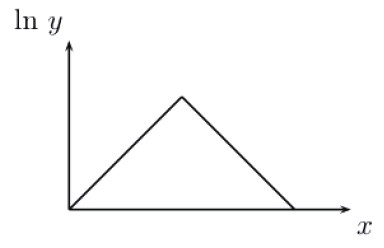
\includegraphics[width=3.5cm]{img/fig01}
\end{center}
Welk van de onderstaande grafieken geeft het verband tussen $x$ en $y$ weer? Omcirkel je antwoord en verklaar kort.\\
\begin{center}
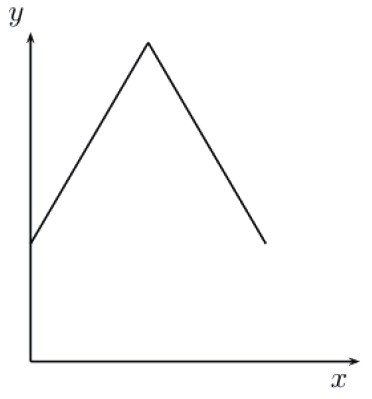
\includegraphics[width=2.9cm]{img/fig05} \hspace{0.2cm} 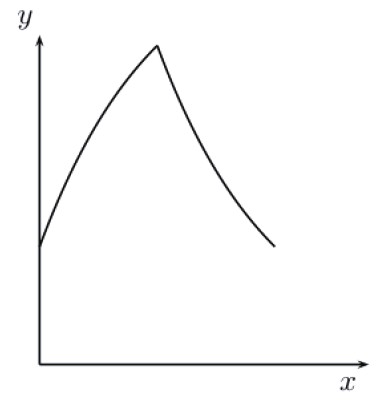
\includegraphics[width=2.9cm]{img/fig03} \hspace{0.2cm} 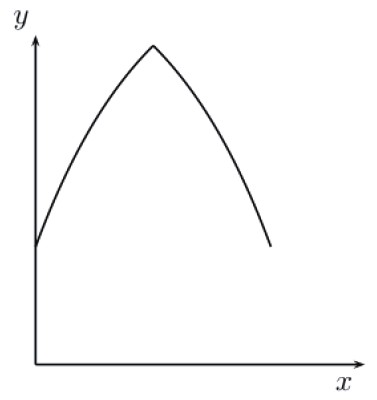
\includegraphics[width=2.9cm]{img/fig04} \hspace{0.2cm} 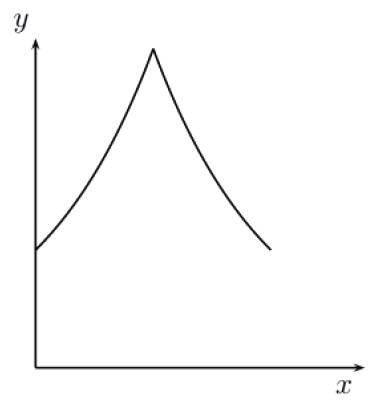
\includegraphics[width=2.9cm]{img/fig02}\hspace{0.2cm} 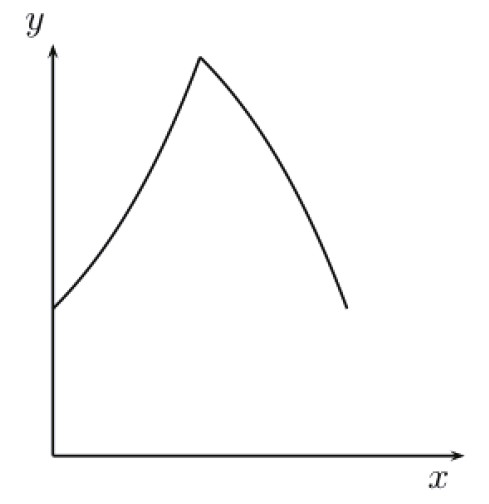
\includegraphics[width=2.9cm]{img/fig06}
\end{center}

\eindewerktekst

\tussentitel{Oplossing}
De vierde grafiek geeft het juiste verband tussen $x$ en $y$ weer.\\ In het eerste deel van de grafiek die het verband tussen $x$ en $\ln y$ geeft, zijn $x$ en $\ln y$ recht evenredig. Stel $\ln y=kx$ met $k>0$. Dan is $y=e^{kx}$. Het eerste deel van de grafiek die het verband tussen $x$ en $y$ geeft, moet dus stijgend exponentieel zijn. Dan blijven enkel nog het vierde en het vijfde antwoordalternatief over. Met een analoge redenering zie je snel in dat het tweede deel van de grafiek exponentieel dalend moet zijn. Het juiste antwoord is dus grafiek 4. 


\tussentitel{Wat maakt deze oefening mooi?}
De verschillende grafische verbanden zien, is niet zo evident. Er zijn verschillende denkstappen nodig. Deze oefening vraagt dus wel wat inzicht, maar het rekenwerk is heel beperkt. Dit zorgt voor een frisse afwisseling met oefeningen waarbij vaak veel rekenvaardigheden nodig zijn. Het is daarom ook een goede toetsvraag: je kunt vrij snel controleren of leerlingen het begrepen hebben en leerlingen die niet zo sterk zijn in rekenvaardigheden lopen niet vast bij het rekenwerk. Vergeet bij toetsen zeker niet een verklaring te vragen zodat het geen gokwerk wordt.

\subsection{Goniometrische functies en goniometrie}

\beginwerktekst{Een goniometrische vergelijking}

Je mag bij deze oefening geen rekentoestel gebruiken.

Bepaal het aantal oplossingen van de vergelijking $\cos (\sin x)=\sin x$ met $x\in ]-\frac{3\pi}{2}, \frac{5\pi}{2}[$. \\Verklaar je antwoord!
\begin{meerkeuze}
    \item minder dan 2
    \item 2
    \item 3
    \item 4
    \item meer dan 4
\end{meerkeuze}


\eindewerktekst
\\ \
\tussentitel{Oplossing}
De oplossing verloopt in twee stappen.\\
We lossen eerst de vergelijking $\cos x=x$ op voor $x\in [-1,1]$. Zonder rekentoestel kunnen we deze niet exact oplossen, maar we kunnen wel een schatting maken door de grafieken van $y=\cos x$ en $y=x$ te schetsen.
\begin{center}
    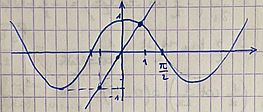
\includegraphics[width=6cm]{img/cosx=x.jpg}
    %\captionof{figure}{}
\end{center}

%\newpage
We lezen af dat er één snijpunt is voor $x$ iets kleiner dan 1 en dus heeft de vergelijking $\cos x=x$ één oplossing. Stel $x\approx 0,8$.\\

In de tweede stap gaan we na hoeveel keer $\sin x$ gelijk wordt aan  $0,8$ voor $x\in ]-\frac{3\pi}{2}, \frac{5\pi}{2}[$. Je kunt dit weer doen via de grafieken, maar het kan ook via de goniometrische cirkel. Je moet dan wel \aanh{twee keer ronddraaien}. De snelle schets hieronder illustreert dit.
\begin{center}
    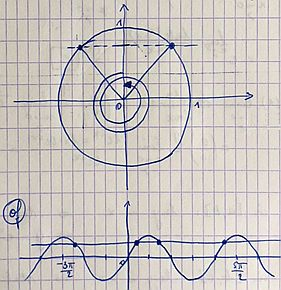
\includegraphics[width=6cm]{img/sinx=0,8.jpg}
    %\captionof{figure}{}
\end{center}
Er zijn dus 4 oplossingen.

\tussentitel{Wat maakt deze oefening mooi?}
Dit is een ongewone goniometrische vergelijking waarbij geen speciale goniometrische formules nodig zijn. Vaak zijn goniometrische vergelijkingen eerder technische oefeningen. Dat is hier niet het geval. Wel zijn er enkele denkstappen die inzicht vragen.\\ Leerlingen moeten eerst beseffen dat er eigenlijk een vergelijking staat van de vorm $\cos x=x$. Dergelijke substituties doen ze regelmatig (denk maar aan bikwadratische vergelijkingen), maar hier zien ze die substitutie niet zo duidelijk. Daarna blijft nog een eenvoudige goniometrische basisvergelijking over, $\sin x=0,8$. Anders dan gewoonlijk moet deze niet opgelost worden, maar moet het aantal oplossingen binnen een bepaald interval berekend worden. De leerlingen moeten beseffen dat dit interval een rol speelt. Heel wat leerlingen maken de fout te denken dat de vergelijking oneindig veel oplossingen heeft. Dat hebben ze immers zo geleerd bij het oplossen van goniometrische vergelijkingen.  Anderen kijken dan weer naar de goniometrische cirkel en zien maar 2 oplossingen voor $\sin x=0,8$ omdat ze vergeten nog een keer \aanh{rond te draaien}. In beide gevallen houden ze geen rekening met het gegeven interval voor $x$.






























%%% Hieronder enkele speciale omgevingen %%%
%%%%%%%%%%%%%%%%%%%%%%%%%%%%%%%%%%%%%%%%%%%%

\newpage
\stopcontents[mainsections]			        % altijd laten staan, opsomming in inhoudstafel enkel tot loep beperken
% bronnen toevoegen
\begin{bronnen}
\item Arnold, S. (2018). \textit{Kissing curves}. Geraadpleegd op 16 november 2018 via\\ www.compasstech.com.au/ARNOLD/geogebra/kissingcurves.html
\item \textit{De doordenker. Een emmer vol met knikkers.} Geraadpleegd op 17 november 2018 via\\ https://rekenbeter.wordpress.com/2011/11/15/doordenker-260/
\item Deloddere, N., e.a. (2009). \textit{Delta Nova 4a (leerweg 5)}. Mechelen: Plantyn. 
\item Hofstede, H. \textit{Gemiddelde toename.} Geraadpleegd op 12 november 2018 via\\
http://www.hhofstede.nl/modules/gemiddeldetoename.htm
\item Kranenborg, J.O. (2018). Raken en snijden. \textit{Euclides}, 93/7.
\item Samenwerkende Vlaamse Universiteiten. (2013). \textit{Ijkingstoets burgerlijk ingenieur-wiskunde-fysica-informatica}. Geraadpleegd op 12 november 2018 via https://www.usolvit.be
\item Talwalkar, P., Mind Your Decisions (28 maart 2018). \textit{VERY HARD South Korean Geometry Problem} [Videobestand]. Geraadpleegd op 7 november 2018 via https://www.youtube.com/
\item van den Broek, L. (2007). \textit{Perspectief. Experimentele uitgave voor Vorm en Ruimte, vwo, wiskunde C.} Geraadpleegd op 12 november 2018 via  http://www.fi.uu.nl/ctwo/lesmateriaaldir/ExperimenteelLesmateriaal/
\end{bronnen}




